\documentclass{report}

\usepackage[T1]{fontenc}
\usepackage[utf8]{inputenc}
\usepackage{times}

\usepackage[font=small,labelfont=bf,tableposition=top]{caption}
\usepackage{graphicx}
\usepackage{natbib} 

\usepackage{amsmath}
\usepackage{amsfonts}
\usepackage{amssymb}
\usepackage{color, soul}
\usepackage{hyperref}
\usepackage{algorithmicx}
\usepackage{algpseudocode}
\usepackage{subfigure}
\usepackage{stmaryrd}

\renewcommand{\vec}[1]{\boldsymbol{{#1}}} 
\newcommand{\duesoon}[1]{{\sethlcolor{green}\hl{#1}}}
\usepackage{mathrsfs}


\newtheorem{theorem}{Theorem}
\newtheorem{acknowledgement}[theorem]{Acknowledgement}
\newtheorem{algorithm}[theorem]{Algorithm}
\newtheorem{axiom}[theorem]{Axiom}
\newtheorem{case}[theorem]{Case}
\newtheorem{claim}[theorem]{Claim}
\newtheorem{conclusion}[theorem]{Conclusion}
\newtheorem{condition}[theorem]{Condition}
\newtheorem{conjecture}[theorem]{Conjecture}
\newtheorem{corollary}[theorem]{Corollary}
\newtheorem{criterion}[theorem]{Criterion}
\newtheorem{definition}[theorem]{Definition}
\newtheorem{example}[theorem]{Example}
\newtheorem{exercise}[theorem]{Exercise}
\newtheorem{lemma}[theorem]{Lemma}
\newtheorem{notation}[theorem]{Notation}
\newtheorem{problem}[theorem]{Problem}
\newtheorem{proposition}[theorem]{Proposition}
\newtheorem{remark}[theorem]{Remark}
\newtheorem{solution}[theorem]{Solution}
\newtheorem{summary}[theorem]{Summary}
\newenvironment{proof}[1][Proof]{\textbf{#1.} }{\ \rule{0.5em}{0.5em}}

\newtheorem{guess}{Definition}
\newcommand{\comment}[1] {}
\newcommand{\Norder} {N}
\newcommand{\order}{\mathcal{O}}
\newcommand{\Npoints} {N_p}
\newcommand{\Nfaces} {N_{f}}
\newcommand{\Nelements} {N_e}

\newcommand{\eps}{\varepsilon}
\newcommand{\Dweak}{\wt{D}}
\newcommand{\diff}[2] {\frac{\partial #1}{\partial #2}}
\newcommand{\dxx}[2] {\frac{\partial^2 #1}{\partial {#2}^2}}
\newcommand{\difft}[2] {\frac{d #1}{d #2}}
\newcommand{\dxxt}[2] {\frac{d^2 #1}{d {#2}^2}}
\newcommand{\lagrange}[1] {\frac{d #1}{dt}}
\newcommand{\lebesgue}{\parallel I \parallel}
\newcommand{\polysp}{\mathcal{P}_N}
\newcommand{\laplacian}{\nabla^2}
\newcommand{\divergence}{\nabla \cdot}
\newcommand{\inte}{\int_{\mbox{\footnotesize ${\Omega_e}$}}}
\newcommand{\intb}{\int_{\mbox{\footnotesize ${\Gamma_e}$}}}
\newcommand{\intce}{\int_{\mbox{\footnotesize ${\widehat{\Omega}_e}$}}}
\newcommand{\intcb}{\int_{\mbox{\footnotesize ${\widehat{\Gamma}_e}$}}}
\newcommand{\intg}{\int_{\mbox{\footnotesize ${\Omega}$}}}
\newcommand{\intgb}{\int_{\mbox{\footnotesize ${\Gamma}$}}}
\newcommand{\intv}{\int_{\mbox{\footnotesize ${\sigma}$}}}
\newcommand{\sumv}{\sum_{K=1}^{N_{\mathrm{lev}}}}
\newcommand{\sumk}{\sum_{L=1}^{K}}
\newcommand{\sumN}{\sum_{i=1}^{N+1}}
\newcommand{\half}{\frac{1}{2}}
\newcommand{\inti}{\int_{\mbox{\footnotesize\sf I}}}
\newcommand{\intbd}{\oint_{\mbox{\footnotesize ${\delta}$\sf D}}}
\newcommand{\intbi}{\oint_{\mbox{\footnotesize ${\delta}$\sf I}}}
\newcommand{\ldnorm}[1]{\left\| #1 \right\|_{\mbox{\footnotesize \sf D}} }
\newcommand{\lonorm}[1]{\left\| #1 \right\|_{\Omega}}
\newcommand{\spc}[1]{\mbox{\sf #1}}
\newcommand{\ope}[1]{{\cal #1}}
\newcommand{\mt}[1]{{\rm #1}}
\newcommand{\dis}{\displaystyle}
\newcommand{\ve}{\varepsilon}
\newcommand{\ov}{\overline}
\newcommand{\wt}{\widetilde}
\newcommand{\wh}{\widehat}
\newcommand{\Dhat}{\widehat{D}}
\newcommand{\be}{\begin{equation}}
\newcommand{\ee}{\end{equation}}
\newcommand{\bea}{\begin{eqnarray*}}
\newcommand{\eea}{\end{eqnarray*}}
\newcommand{\Jace}{J^{(e)}}
\newcommand{\Jacl}{J^{(l)}}
\def\bepsilon{\mbox{\boldmath $\epsilon $}}
\def\bpsi{\mbox{\boldmath $\psi $}}
\def\bphi{\mbox{\boldmath $\phi $}}
\def\bmu{\mbox{\boldmath $\mu $}}
\def\Et{ \tilde{E} }
\def\Ht{ \tilde{H} }
\def\sdot{ \dot{\sigma} }

\newcommand{\fstar}{f^{(*)}}

\DeclareMathOperator{\Span}{span}
\DeclareMathOperator{\Dim}{dim}

\newcommand{\polyquad}{\mathcal{Q}_{N}}
\newcommand{\polyP}{\mathcal{P}_{N}}
\newcommand{\polyPnpm}{\mathcal{P}_{(N+M)}}
\newcommand{\polyPd}{\mathcal{P}_{d}}
\newcommand{\polyPnm}{\mathcal{P}_{N,M}}
\newcommand{\polyPn}{\mathcal{P}_{N,0}}
\newcommand{\transpose}{^{\mathcal{T}}}

\newcommand{\vecQ}{\vec{Q}}
\newcommand{\vecQe}{\vec{Q}^{(e)}}
\newcommand{\vecFe}{\vec{\mathcal{F}}^{(e)}}
\newcommand{\statevec}{\vec{Y}}
\newcommand{\statevecN}{\vec{Y}_N^{(e)}}
\newcommand{\statestage}{\vec{\mathcal{Y}}}
\newcommand{\Ftensor}{\vec{F}(\qvector)}
\newcommand{\FtensorN}{\vec{F}\left( \qvectorN \right)}
\newcommand{\FtensorStar}{\vec{F}\left( \qvector_N^{(e,k)} \right)}
\newcommand{\Svector}{S(\qvector)}
\newcommand{\SvectorN}{S \left( \qvectorN \right)}
\newcommand{\qref}{\vec{q}_0}
\newcommand{\qvectorb}{\vec{q}_b}
\newcommand{\qtt}{\vec{q}_{tt}}
\newcommand{\qhat}{\widehat{\vec{q}}}
\newcommand{\qhatb}{\widehat{\vec{q}}_b}
\newcommand{\qelem}{q^{(e)}}
\newcommand{\rhoref}{\rho_0}
\newcommand{\piref}{\pi_0}
\newcommand{\Thetaref}{\Theta_0}
\newcommand{\Gref}{G_0}
\newcommand{\Tref}{T_0}
\newcommand{\thetaref}{\theta_0}
\newcommand{\Pref}{{P}_0}
\newcommand{\Eref}{{E}_0}
\newcommand{\Href}{{h}_0}
\newcommand{\rhohat}{\widehat{\rho}}
\newcommand{\pihat}{\widehat{\pi}}
\newcommand{\Phat}{\widehat{P}}
\newcommand{\uvechat}{\widehat{{\mbox{\boldmath$u$\unboldmath}}}}
\newcommand{\uhathat}{\widehat{\widehat{{\mbox{\boldmath$u$\unboldmath}}}}}
\newcommand{\Uhat}{\widehat{{\mbox{\boldmath$U$\unboldmath}}}}
\newcommand{\Uhathat}{\widehat{\widehat{{\mbox{\boldmath$U$\unboldmath}}}}}
\newcommand{\thetahat}{\widehat{\theta}}
\newcommand{\Thetahat}{\widehat{\Theta}}
\newcommand{\Ehat}{\widehat{E}}
\newcommand{\uhat}{\widehat{u}}
\newcommand{\vhat}{\widehat{v}}
\newcommand{\what}{\widehat{w}}
\newcommand{\pitt}{\pi_{tt}}
\newcommand{\rhott}{\rho_{tt}}
\newcommand{\Ett}{E_{tt}}
\newcommand{\Utt}{\vec{U}_{tt}}
\newcommand{\uvectt}{\vec{u}_{tt}}
\newcommand{\utt}{u_{tt}}
\newcommand{\vtt}{v_{tt}}
\newcommand{\wtt}{w_{tt}}
\newcommand{\Ptt}{P_{tt}}
\newcommand{\vecPtt}{\vec{P}_{tt}}
\newcommand{\Thetatt}{\Theta_{tt}}
\newcommand{\thetatt}{\theta_{tt}}
%Projector Matrices
\newcommand{\projmatrix}{\vec{\mathcal{P}}}
\newcommand{\qmatrix}{\vec{\mathcal{Q}}}
\newcommand{\pcmatrix}{\vec{\mathcal{P}}_C}
\newcommand{\Cmatrix}{\left(\vec{\mathcal{C}}^{(e,f)}\right)\transpose}
\newcommand{\Dmatrix}{\vec{D}^{(e)}}
\newcommand{\Dwmatrix}{\wt{\vec{D}}^{(e)}}
\newcommand{\Mmatrix}{M^{(e)}}
\newcommand{\Fmatrix}{\vec{F}^{(e,l)}}
\newcommand{\Gmatrix}{\mathcal{G}}
\newcommand{\Umatrix}{\mathcal{U}^{(e,f)}}
\newcommand{\amatrix}{\vec{\mathcal{A}}}
\newcommand{\rmatrix}{\vec{\mathcal{R}}}
%Vectors
\newcommand{\nvector}{\wh{\vec{n}}_{\Gamma}}
\newcommand{\nhat}{\wh{\vec{n}}}
\newcommand{\ivector}{\wh{\vec{i}}}
\newcommand{\jvector}{\wh{\vec{j}}}
\newcommand{\kvector}{\wh{\vec{k}}}
\newcommand{\rvector}{\wh{\vec{r}}}
\newcommand{\svector}{\wh{\vec{s}}}
\newcommand{\tvector}{\wh{\vec{t}}}
\newcommand{\vvector}{\wh{\vec{v}}}
\newcommand{\Qvector}{\vec{Q}}
%Vectors
\newcommand{\ur}{{u}^{(r)}}
\newcommand{\us}{{u}^{(s)}}
\newcommand{\ut}{{u}^{(t)}}
\newcommand{\urtt}{{u}_{tt}^{(r)}}
\newcommand{\ustt}{{u}_{tt}^{(s)}}
\newcommand{\uttt}{{u}_{tt}^{(t)}}
\newcommand{\urhat}{\widehat{u}^{(r)}}
\newcommand{\ushat}{\widehat{u}^{(s)}}
\newcommand{\uthat}{\widehat{u}^{(t)}}
%Other Operators
\newcommand{\grad}{\vec{\nabla}}
\newcommand{\Grad}{\vec{\nabla}}
\newcommand{\Dskew}{\mathcal{D}}

\def\bepsilon{\mbox{\boldmath $\epsilon $}}
\def\bpsi{\mbox{\boldmath $\psi $}}
\def\bphi{\mbox{\boldmath $\phi $}}
\def\bmu{\mbox{\boldmath $\mu $}}
\def\Et{ \tilde{E} }
\def\Ht{ \tilde{H} }
\def\sdot{ \dot{\sigma} }
%\renewcommand{\thetable}{\Roman{table}}
%\renewcommand{\thefigure}{\arabic{figure}}

%\DeclareMathOperator{\Span}{span}
%\DeclareMathOperator{\Dim}{dim}

%Editing Commands
\newcommand{\here}{ \textcolor{red}{YOU ARE HERE}}

%Time-Integration
\newcommand{\dt}{{\Delta t}}
\newcommand\ST{\rule[-0.75em]{0pt}{2em}}
\newcommand{\Sfunction}{\mathcal{S}}
\newcommand{\Lfunction}{\mathcal{L}}
\newcommand{\Nfunction}{\mathcal{N}}

%DG Operators
\newcommand{\average}[1]{ \left\{ #1 \right\} }
\newcommand{\jump}[1]{ \llbracket #1 \rrbracket }

%HDG Matrices
\newcommand{\CCmatrix}{\mathcal{C}^{(e,k)}}
\newcommand{\Jmatrix}{\mathcal{J}^{(e,k)}}
\newcommand{\DDmatrix}{\wt{D}^{(e)}}
\newcommand{\SSvector}{\mathcal{S}(q)}
\newcommand{\cghdg}{cg\underline{\hspace{0.15cm}}to\underline{\hspace{0.15cm}}hdg}
%\newcommand{\ul}{\underline{\hspace{0.15cm}}}
\newcommand{\RRmatrix}{\mathcal{R}}

%Clima specific variables
\newcommand{\etotal}{e^{\mathrm{tot}}}
\newcommand{\Etotal}{E^{\mathrm{tot}}}
\newcommand{\Fvector}{\vec{\mathcal{F}}}
\newcommand{\Pvector}{\vec{\mathcal{P}}}
\newcommand{\Fadv}{\vec{\mathcal{F}}^{\mathrm{adv}}}
\newcommand{\Fndf}{\vec{\mathcal{F}}^{\mathrm{ndf}}}
\newcommand{\Fdiff}{\vec{\mathcal{F}}^{\mathrm{diff}}}
\newcommand{\Tvector}{\vec{\mathcal{T}}}
\newcommand{\Source}{\vec{\mathcal{S}}}

\newcommand{\fxg}[1]{\textcolor{cyan}{FXG: #1}}


\usepackage[inline]{enumitem}
\usepackage{hyperref}
\usepackage{comment}
\hypersetup{
    colorlinks=true,
    linkcolor=blue,
    citecolor=blue,
    filecolor=cyan,      
    urlcolor=cyan,
}

\title{CLIMA Land Model} 

\author{ }

\begin{document}

\maketitle
\tableofcontents

\chapter{Purpose, Goals, and Non-Goals}

\section{Overview}

This document describes the scientific concepts underlying the CLIMA land model. It lays out a consistent set of equations governing components of the land model such as soil, snow, and vegetation, and it discusses the boundary conditions through which the land model couples to the atmosphere. The land model is built upon these concepts and equations and is designed to be coupled to the CLIMA atmosphere model or run in standalone mode (e.g., driven by reanalysis data). Because the land model is part of a climate model, conservation of energy, water, and carbon are essential, both within the land model and in exchanges with the atmosphere. Figure~\ref{f:land_model_schematic} provides a schematic of the land model components and how they interact with each other and with the atmosphere and ocean models. Table~\ref{tab:LM-modules} summarizes the model components and their inputs, outputs, and functional requirements, which are discussed in detail in this document.\hl{[update figure and table]}
\begin{figure}[htb]
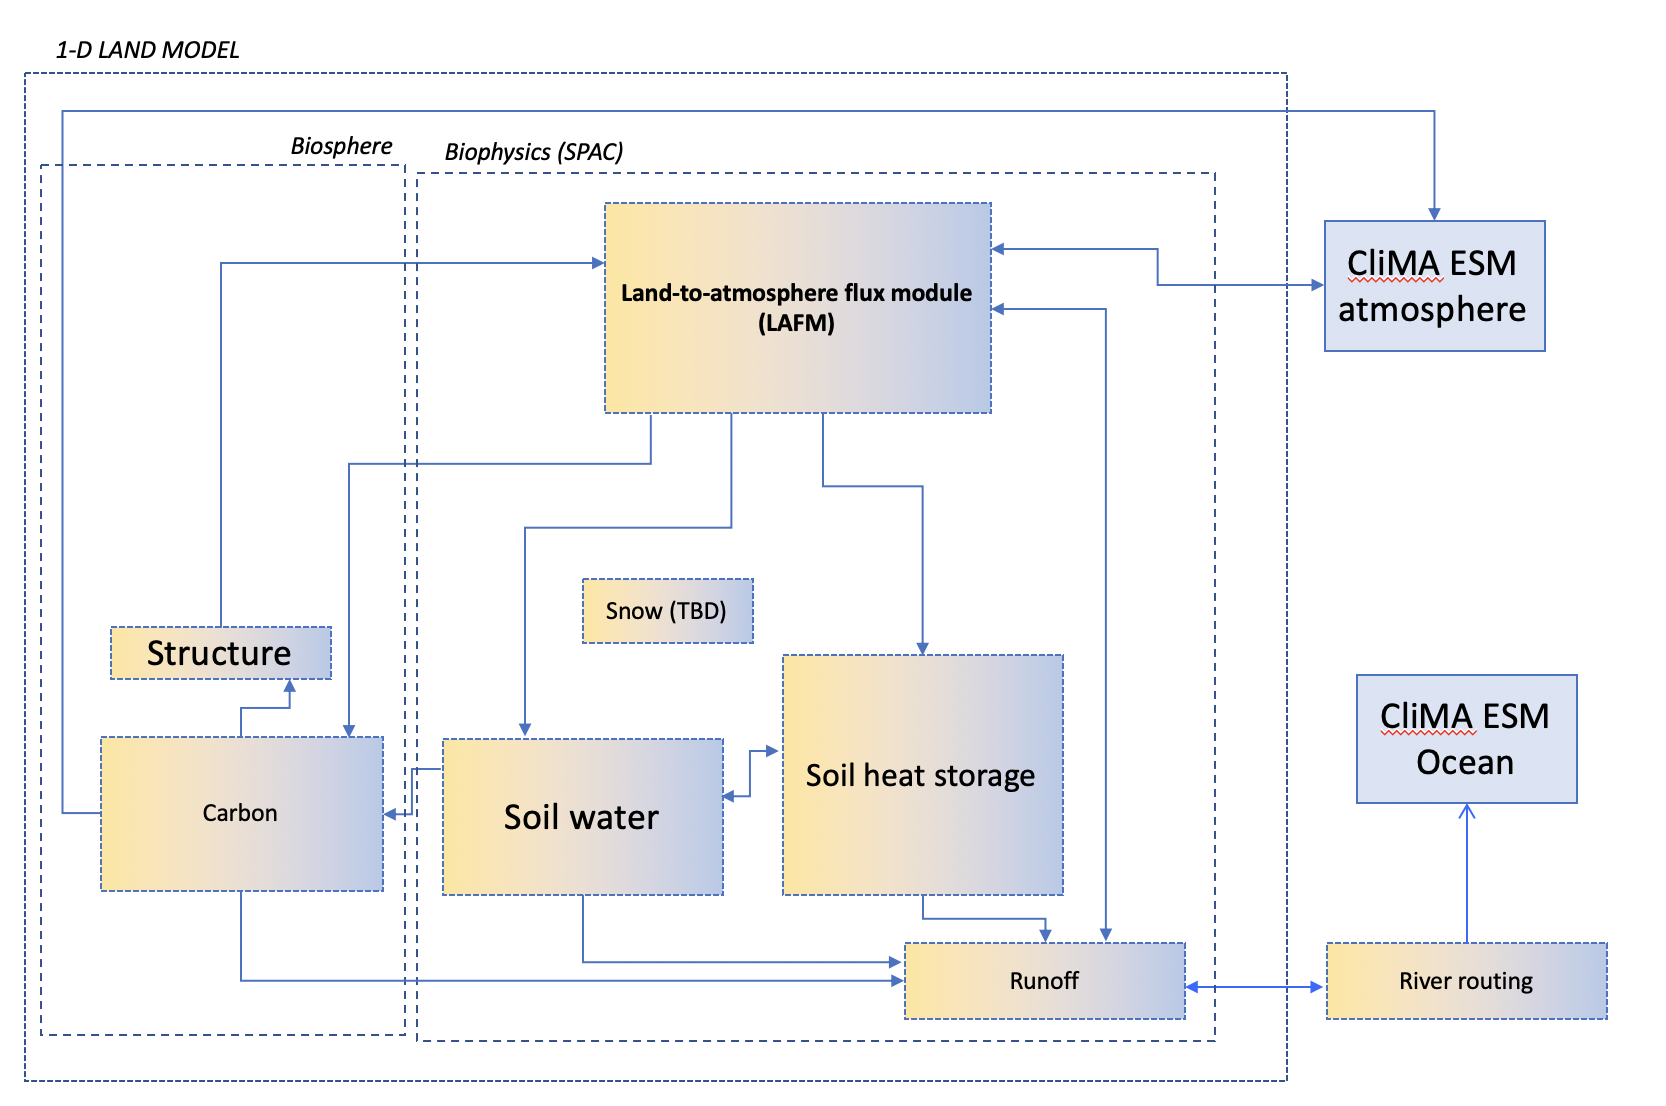
\includegraphics[width=10cm,height=10cm,keepaspectratio]{CLIMA-land/LM_figures/JPLCLIMA_LM_DESIGN_20191115.png}
\caption{Schematic of land model components and their internal and external dependencies. Model components interact with each other; for example, the canopy model interacts with the soil model through source/sink terms representing processes such as water uptake by roots, and it interacts with turbulent fluxes in the atmospheric near-surface layer through exchange of momentum, energy, and water. \hl{[ALL: please comment + suggest improvements; Pierre's comment: SPAC should include all biophysics, re-name/re-arrange/simplify boxes]}}
\label{f:land_model_schematic}
\end{figure}
% Please add the following required packages to your document preamble:
% \usepackage{graphicx}
\begin{table}[]
\resizebox{\textwidth}{!}{%
\begin{tabular}{|l|l|l|l|}
\hline
Module [code]         & Input requirements [From]                                                                & Output requirements                                                       & Module requirements                      \\ \hline
Carbon [C]            & \begin{tabular}[c]{@{}l@{}}GPP [F], \\ Soil water profile [W], \\ Soil temperature profile [E]\end{tabular}                                                               & \begin{tabular}[c]{@{}l@{}}Carbon states\\ (Biomass, inc. foliar, roots, wood;\\ Dead organic C) \\ Carbon fluxes \\ (respiration, disturbance fluxes)\end{tabular} & \begin{tabular}[c]{@{}l@{}}The carbon module will calculate \\ internal land biosphere carbon transfers \\ (allocation, mortality, mineralization), \\ and gross land-atmosphere C fluxes \\ (respiration, fires)\end{tabular} \\ \hline

Structure [S]         & Biomass [C]                                                             & \begin{tabular}[c]{@{}l@{}}Biophysical states:\\ Canopy height, Chlorophyll, \\Root profile, LMA\end{tabular}                                                        &                                                                   \\ \hline
Soil water [H]        & \begin{tabular}[c]{@{}l@{}}Soil freeze/thaw state [E] \\ Precipitation [A]\\ Evaporation [F], \\ Transpiration (vertically resolved), \\ root profile [S]\end{tabular} &
\begin{tabular}[c]{@{}l@{}}
Vertical soil water states\\Soil water fluxes\\Runoff\end{tabular}                                                                                                                  & \begin{tabular}[c]{@{}l@{}}Module will calculate vertical \\ water flow in soil Darcy’s law, \\ Richards equations, hydraulic \\redistribution,  runoff, etc.\end{tabular}                                                     \\ \hline
Soil heat storage [E] & Soil water [H], Precip. temp [A]
& 
\begin{tabular}[c]{@{}l@{}}
Vertical temperature profile\\
Runoff temperature       \end{tabular}                                               &                                                                                                \\ \hline
%%%%%%(SPAC-Flux)%%%%%
\begin{tabular}[c]{@{}l@{}}
Land-to-atmosphere\\ fluxes [F]  \\
(previously SPAC-Flux)
\end{tabular}

        & \begin{tabular}[c]{@{}l@{}}Atmospheric variables [A], \\ Biophysical states[S], \\ Soil water profile [H], \\ Soil energy profile [E],\end{tabular}                   & \begin{tabular}[c]{@{}l@{}}Land-surface Fluxes\\ GPP, evapotranspiration, H, $\lambda$E, radiative fluxes \end{tabular}                                 & 

\begin{tabular}[c]{@{}l@{}} Canopy P interception\\ Radiative transfer in canopy     \end{tabular}                                                        \\ \hline

River routing [R]        & \begin{tabular}[c]{@{}l@{}} Soil runoff [H], \\ CliMA Ocean [O] \end{tabular}                             & \begin{tabular}[c]{@{}l@{}} River Discharge\end{tabular}                                             &                                     \\ \hline \hline \hline


CliMA Atmosphere [A]        & \begin{tabular}[c]{@{}l@{}}Land surface fluxes [F], \\ Land biosphere fluxes [C]\end{tabular}                             & \begin{tabular}[c]{@{}l@{}}Atmospheric variables [for land]\\ Radiative fluxes, precipitation, temperature, humidity,\end{tabular}                                             &                                     \\ \hline

CliMA Ocean [O]        & \begin{tabular}[c]{@{}l@{}}River discharge [R] \end{tabular}                             & \begin{tabular}[c]{@{}l@{}} Ocean variables (for land) Sea Level\end{tabular}                                             &                                     \\ \hline
\end{tabular}}
\caption{\label{tab:LM-modules}Overview of inputs, outputs, and functional requirements of land model components.}
\end{table}

Chapter~\ref{c:soil} begins with a description of the soil model and its treatment of the energy and water balance of soil. \hl{[add rest of overview]}.

\section{Goals}

\begin{itemize}
    \item Provide a complete and self-contained documentation of the scientific concepts underlying the land model.
    \item Establish a consistent notation for the governing equations, which may guide data structures and variable names in the code.
    \item Establish a consistent set of approximations for the governing equations that allow the land model to be used both on climate model scales (tens of kilometers and larger) and large-eddy simulation (LES) scales (kilometers and smaller).
    \item Describe boundary conditions that ensure conservation of energy, water, and tracer (e.g., carbon) masses during exchanges with other climate model components, while treating the interfacial layer (e.g., near-surface turbulence in the atmosphere) consistently across model components.
    \item Harmonize equations and boundary conditions to facilitate coupling with the \href{https://github.com/climate-machine/Design-Docs/blob/master/CLIMA-atmos/}{CLIMA atmosphere} model.
    \item Lay out the concepts in a way that can be directly translated into code.
    \item Document benchmark cases for testing the land model.
\end{itemize}

\section{Non-Goals}

\begin{itemize}
    \item Discuss software architecture and data structures.
    \item Discuss numerical methods in detail.
    \item Discuss implementation details such as variable names and computational aspects.
\end{itemize}
These are covered in the separate design documents, on \href{https://github.com/climate-machine/Design-Docs/tree/master/CLIMA-numerics}{numerical methods} and software. \hl{[TBW, link]}.

\chapter{Soil}\label{c:soil}

The soil model represents the transport of energy and moisture in soil, links them to atmospheric boundary conditions above, and provides water input for a runoff models (e.g., rivers). Vegetation is linked to the soil model through root extraction, which represents water sources and sinks in soil, and through modulation of radiation reaching the top of the soil.  This chapter describes the energy and water balances in soil and how atmospheric boundary conditions and vegetation link to them.

\section{Composition of Soil}

\subsection{Bulk Soil}

We take soil to consist of a dry soil matrix (composed of sand, clay, rock, etc.) with pore spaces that may contain liquid water, ice, and gases (e.g., air). The bulk density of the soil mixture is $\rho$ ($\mathrm{kg~m^{-3}}$). The composition of soil is characterized by mass fractions (mass of constituent divided by total mass of soil):
\begin{itemize}
    \item $q_{ds}$: mass fraction of dry soil,
    \item $q_l$: mass fraction of liquid water,
    \item $q_i$: mass fraction of ice,
    \item $q_w = q_l + q_i$: mass fraction of total water (liquid and ice).
\end{itemize}
We neglect the small mass (but not the volume) of gases in pore spaces, so that this enumerates all constituents of soil that contribute to soil mass; therefore, 
\[
q_{ds} + q_l + q_i = q_{ds} + q_w = 1.
\]

Because the primary constituents of soil are essentially incompressible, the composition of soil is commonly expressed in terms of volume fractions (e.g., volume of liquid water per volume of soil). The volume fractions $\theta_{\cdot}$ are related to the mass fractions $q_{\cdot}$ through
\begin{subequations}\label{e:vol_fractions}
\begin{align}
    \theta_{ds} &= \frac{q_{ds} \rho}{\rho_{ds}} \\
    \theta_l &= \frac{q_l \rho}{\rho_l}, \\
    \theta_i &= \frac{q_i \rho}{\rho_i}, \\
    \theta_w &= \theta_l + \theta_i.
\end{align}
\end{subequations}
Here, $\rho_{ds}$ is the particle density of dry soil (i.e., the density of the soil particles alone, without pore spaces), and $\rho_l$ and $\rho_i$ are the densities of liquid water and ice, respectively. We take liquid water to be incompressible, and the densities $\rho_l$ of liquid and $\rho_i$ of ice to be constant. We summarize the water content of soil by the vector $\vec{\theta} = (\theta_l, \theta_i)$.

While the mass fractions of dry soil and water sum to one, the volume fractions do not: Gases, which are assumed to have zero mass, occupy a volume fraction $\theta_g = 1 - (\theta_{ds} + \theta_w)$. Gases, liquid water, and ice occupy pore spaces in the soil matrix. The volume fraction of pore spaces that can be filled with either gas or water is the porosity 
\begin{equation}\label{e:porosity}
    \nu_p = \theta_g + \theta_w =  1 - \theta_{ds}.
\end{equation}
The porosity is the volume fraction filled with gas when the soil is dry ($\theta_w=0$), or it is the volume fraction occupied by water when all voids are filled with liquid water ($\theta_g = \theta_i = 0$). 

\subsection{Dry Soil}

The dry soil portion of the bulk soil in turn consists of constituents such as mineral soil, gravel, organic matter, bedrock, which all have different thermodynamic and hydraulic properties.  Let $\nu_{i}$ indicate the volume fraction of constituent $\chi_i$ in the total volume of soil, with $\chi_i$ labeling the constituents, for example,
\[
\chi_i \in \{ {\mathrm{sand}}, {\mathrm{clay}}, {\mathrm{silt}}, {\mathrm{gravel}}, \mathrm{organic~matter}, {\mathrm{bedrock}} \}.
\]
We include bedrock in the soil constituents to be able to directly apply our soil model in bedrock, simply by modifying location-specific thermodynamic and hydraulic parameters. If the $\nu_i$'s enumerate all constituents of dry soil, the volume fractions sum to the total dry-soil volume fraction $1-\nu_p$,
\[
\sum_i \nu_{i} = 1-\nu_p.
\] 
We use the vector $\vec{\nu} = \{\nu_p, \nu_i\}$ to summarize the composition of dry soil, including its porosity $\nu_p$.

\section{Heat Capacity of Soil}

\subsection{General Formulation}

The specific heat capacity of soil (heat capacity per unit mass, $\mathrm{J~kg^{-1}~K^{-1}}$) is the mass-weighted sum of the specific heat capacities of the constituents
\begin{equation}\label{e:soil_specific_heat}
    c_s = (1-q_w) c_{ds} + q_l c_{l} + q_i c_{i},
\end{equation}
where we have used $q_{ds} = 1 - q_w$ and the specific heat capacities of the constituents are:
\begin{itemize}
    \item $c_{ds}$: Specific heat capacity of dry soil,
    \item $c_l$: Specific heat capacity of liquid water,
    \item $c_i$: Specific heat capacity of ice.
\end{itemize}
Consistent with neglecting the mass of the gas constituents, we neglect their contribution to the soil specific heat capacity.

The specific heat capacity of dry soil depends on spatially varying soil properties (discussed below). We take the specific heat capacities of liquid water and ice to be constants, consistent with the thermodynamics of the  \href{https://github.com/climate-machine/Design-Docs/blob/master/CLIMA-atmos/}{CLIMA atmosphere} model. These constants should be chosen to be the same in atmosphere, ocean, land, and other models; they are set in the \href{https://github.com/climate-machine/CLIMA/tree/master/src/Common/PlanetParameters}{PlanetParameters} module.

Because, as is common, we use volume fractions to characterize the composition of the soil, we also use the volumetric heat capacities (heat capacities per unit volume, $\mathrm{J~m^{-3}~K^{-1}}$):
\begin{subequations}\label{e:vol_heat_capacities}
\begin{align}
    \tilde{c}_{ds} &= \rho_{ds} c_{ds},\\
    \tilde{c}_{l} &= \rho_{l} c_{l},\\
    \tilde{c}_{i} &= \rho_{i} c_{i}.
\end{align}
\end{subequations}
In terms of volume fractions of constituents, the combined volumetric heat capacity of soil is the weighted mean
\begin{equation}\label{e:soil_spec_heat_volume_0}
    \tilde c_s = \rho c_s = (1-\nu_p) \tilde c_{ds} + \theta_l \tilde c_l + \theta_i \tilde c_i.
\end{equation}
This expression for the volumetric heat capacity follows by substituting the definitions of volume fractions \eqref{e:vol_fractions}, porosity \eqref{e:porosity}, and volumetric heat capacities \eqref{e:vol_heat_capacities} into the definition of the specific heat capacity of soil \eqref{e:soil_specific_heat}. Instead of referring the heat capacity of dry soil to a unit volume of solid soil only (excluding the pore space volume), it is convenient to use a bulk heat capacity of a volume of dry soil that includes the pore space volume:
\begin{equation}\label{e:bulk_dry_heat_capacity0}
    \check{c}_{ds} = (1-\nu_p) \tilde{c}_{ds}.
\end{equation}
In terms of this bulk volumetric heat capacity of dry soil, the  becomes
\begin{equation}\label{e:soil_spec_heat_volume}
    \tilde c_s (\vec{\theta}; \vec{\nu}) = \check c_{ds} + \theta_l \tilde c_l + \theta_i \tilde c_i,
\end{equation}
which is a function of the soil composition: it depends on water content  $\vec{\theta}$ (a model variable) and parametrically on the dry-soil composition $\vec{\nu}$. The expression \eqref{e:soil_spec_heat_volume} makes it clear that the heat capacity of soil increases with increasing moisture content because filling pore spaces with soil water reduces the thermal resistance between dry soil particles. (Here and throughout this document, we use tilde and check accents to indicate thermodynamic quantities referenced to volume rather than mass.) 

\subsection{Heat Capacity of Dry Soil}

The volumetric heat capacity of dry soil is commonly approximated as the weighted mean of the volumetric heat capacities of mineral soil, gravel, organic matter, bedrock, and possibly other constituents \citep{Farouki81a}. If ${\tilde c}_{\chi_i}$ denotes the volumetric heat capacity of constituent $\chi_i$, the volumetric heat capacity of dry soil is the weighted mean 
\begin{equation}\label{e:dry_soil_heat_capacity}
\tilde{c}_{ds} (\vec{\nu}) = (1-\nu_p)^{-1} \sum_i \nu_{i} {\tilde c}_{\chi_i}.
\end{equation}
This is the volumetric heat capacity of the solid components of dry soil only, that is, excluding the pore space volume. The bulk heat capacity of a volume of dry soil that includes the pore space volume is
\begin{equation}\label{e:bulk_dry_heat_capacity}
    \check{c}_{ds} (\vec{\nu})  = (1-\nu_p) \tilde{c}_{ds} = \sum_i \nu_{i} {\tilde c}_{\chi_i}.
\end{equation}
This bulk dry heat capacity is commonly tabulated. 

The particle density of dry soil follows analogously as the weighted mean of the constituent particle densities $\rho_{\chi_i}$:
\begin{equation}\label{d:dry_soil_density}
    \rho_{ds}(\vec{\nu})  = (1-\nu_p)^{-1} \sum_i \nu_{i} {\rho}_{\chi_i}.
\end{equation}
This gives the bulk soil density  
\begin{equation}\label{e:bulk_density}
\rho (\vec{\theta}; \vec{\nu}) = (1-\nu_p) \rho_{ds} + \theta_l \rho_l + \theta_i \rho_i,
\end{equation}
which follows from the definition of the volume fractions \eqref{e:vol_fractions} and of porosity \eqref{e:porosity}. 

Sources of the data needed to specify soil composition $\vec{\nu}$ and heat capacities $\check c_{ds}$ are listed in section~\ref{s:soil_data}.

\section{Thermodynamic State of Soil}

\subsection{Internal Energy}

We characterize the thermodynamic state of soil by its internal energy. The specific internal energy (energy per unit mass, $\mathrm{J~kg^{-1}}$) is the mass-weighted mean of the constituent specific internal energies of dry soil $I_{ds}$, liquid water $I_l$, and ice $I_i$,
\begin{equation}\label{e:energy_soil}
    I = (1-q_w) I_{ds} + q_l I_l + q_i I_i.
\end{equation}
Gases are again neglected, consistent with neglecting their mass. The specific internal energies of the constituents depend on the temperature $T$ of the constituents (which are assumed to be in local thermal equilibrium, so they have the same temperature in any one location) and the specific heat capacities:
\begin{subequations}\label{e:soil_internal_energies}
\begin{align}
I_{ds}(T; \vec{\nu}) & = c_{ds}(\vec{\nu}) (T - T_0),  \\
I_l(T) & = c_{l} (T - T_0), \\
I_i(T) & = c_{i} (T - T_0) - I_{i,0}.
\end{align}
\end{subequations}
The temperature $T_0$ is a reference temperature at which the specific internal energy of soil and liquid water are taken to vanish, and $I_{i,0}$ is the difference in specific internal energy between ice and liquid water at $T_0$. Equating internal energies and enthalpies of liquid water and ice, we approximate the specific internal energy difference $I_{i,0}$ by the specific enthalpy difference at $T_0$, which is the specific latent heat of fusion $L_{f,0}$ at $T_0$: 
\begin{equation}
    I_{i,0} = L_{f,0}.
\end{equation} 
These definitions for the internal energy of soil are consistent with those for the \href{https://github.com/climate-machine/Design-Docs/blob/master/CLIMA-atmos/}{CLIMA atmosphere} model. The reference temperature $T_0$ is arbitrary but the specific latent heat of fusion must be chosen at $T_0$. The thermodynamic properties of water must be chosen to be the same for soil, atmosphere, and other model component, to ensure thermodynamic consistency. 

For the soil model, it is again convenient to use internal energies per unit volume ($\mathrm{J~m^{-3}}$) rather than the internal energies per unit mass. The internal energies per unit volume are related to the specific internal energies by
\begin{subequations}
\begin{align}
    \tilde I_{ds} &= \rho_{ds} I_{ds},\\
    \tilde I_{l}  &= \rho_{l} I_{l},\\
    \tilde I_{i}  &= \rho_{i} I_{i}.
\end{align}
\end{subequations}
Using the fact that the specific heat capacity of soil \eqref{e:soil_specific_heat} is the weighted mean of those of the constituents, together with the relation \eqref{e:soil_spec_heat_volume} for the volumetric specific heat, and the definition \eqref{e:vol_fractions} of the volume fractions, the total internal energy per unit volume can be written as
\begin{equation}\label{e:vol_internal_energy}
\begin{split}
    \tilde I(T, \vec{\theta}; \vec{\nu})  &= \rho I 
    = \theta_{ds} \tilde I_{ds}(T; \vec{\nu}) + \theta_l  \tilde I_l(T) + \theta_i  \tilde I_i(T)\\
    &= \tilde{c}_s(\vec{\theta}; \vec{\nu}) (T - T_0) - \theta_i \rho_i L_{f,0}.
\end{split}
\end{equation}
The internal energy $\tilde I$ of soil depends on temperature $T$ and, through the volumetric specific heat $\tilde c_s(\vec{\theta}; \vec{\nu})$, on water content $\vec{\theta}$ and, parametrically, on the dry-soil composition $\vec{\nu}$, which is a location-dependent parameter vector (see section~\ref{s:soil_data}).

\subsection{Temperature}

Given the internal energy $\tilde I$ and composition ($\vec{\theta}; \vec{\nu}$) of the soil, the definition \eqref{e:vol_internal_energy} can be inverted go give the soil temperature
\begin{equation}\label{e:temperature_from_I}
    T = T_0 + \frac{\tilde{I} + \theta_i \rho_i L_{f,0}}{\tilde{c}_s(\vec{\theta}; \vec{\nu})}.
\end{equation}
Thus, we can use the internal energy $\tilde I$ as a prognostic variable in a soil model and can from that and from knowledge of the composition ($\vec{\theta}; \vec{\nu}$) of the soil obtain the temperature $T$. If only the total water volume fraction $\theta_w$ is known but not its temperature-dependent partitioning into liquid $\theta_l$ and ice $\theta_i$, solving for temperature given internal energy $\tilde I$ is a nonlinear problem that must be solved iteratively. 

Using internal energy rather than temperature as a prognostic variable is advantageous because internal energy, unlike temperature, is conserved when water freezes or thaws. Thus, internal energy is unaffected by reversible phase transitions of water and remains continuous at freezing/thawing fronts.

\section{Energy Balance}

\subsection{Conservation Law}

The conservation law for internal energy is
\begin{equation}\label{e:energy_conservation}
    \frac{\partial \tilde I}{\partial t} =  - \divergence \bigl(\vec{\tilde J} + \vec{\tilde D}\bigr) + \tilde Q - \divergence \vec{\tilde F}_R.
\end{equation}
Internal energy changes by divergence of conductive heat fluxes $\vec{\tilde J}$ and of energy fluxes $\vec{\tilde D}$ carried by moving (diffusing) water. Additionally, it can change by external heat sources/sinks $\tilde Q$ ($\mathrm{W~m^{-3}}$)---for example, metabolic heat from soil microbes---and divergence of any radiative energy fluxes $\vec{\tilde F}_R$ that penetrate into the soil. (Radiative fluxes penetrating into the soil are generally not resolved in soil models and only enter as upper boundary conditions, so that their flux divergence in the soil vanishes.\footnote{The radiative energy flux also appears in the \protect\href{https://github.com/climate-machine/Design-Docs/blob/master/CLIMA-atmos/}{CLIMA atmosphere} model, where it is referenced to unit mass, $\vec{F}_R$ ($\mathrm{W~m~kg^{-1}}$), with $\vec{\tilde F}_R = \rho \vec{F}_R$.}) Consistent with the internal energy being referenced to a unit volume, the energy fluxes $\vec{\tilde J}$, $\vec{\tilde D}$, and $\vec{\tilde F}_R$ are referenced to a unit area ($\mathrm{W~m^{-2}}$). 

Because vertical variations in soil generally are much greater than horizontal variations, the derivative operator in all current Earth system models is approximated by its vertical component ($\nabla \approx \partial/\partial z$), reducing the conservation law \eqref{e:energy_conservation} to a one-dimensional partial differential equation. However, in what follows we keep the notation general, to develop the model setup to be generally usable in 3D as well as 1D. 

The conductive heat flux is given by Fourier's law as
\begin{equation}
    \vec{\tilde J} = - \kappa \grad T, 
\end{equation}
where $\kappa = \kappa(\vec{\theta}; \vec{\nu})$ ($\mathrm{W~m^{-1}~K^{-1}}$) is the thermal conductivity of soil, which we take to be isotropic (scalar) and which depends on the soil composition $(\vec{\theta}; \vec{\nu})$. The energy flux carried by diffusion of water is 
\begin{equation}
    \vec{\tilde D} = \tilde I_l \vec{\tilde d}_{l},
\end{equation}
where the diffusive flux of liquid water $\vec{\tilde d}_{l}$ is discussed further in section~\ref{s:water_balance}. 

The conservation law \eqref{e:energy_conservation} for internal energy in soil is approximately the conservation law for total energy. Kinetic energy and gravitational potential energy in principle also contribute to the total energy. But the kinetic energy of water motion is orders of magnitude smaller than the internal energy. And conversion into internal energy of gravitational potential energy associated with water motion likewise is negligible. Hence, the internal energy conservation law closely approximates the total energy conservation law. 

Table~\ref{t:thermodynamics_soil} summarizes the thermodynamic quantities entering the energy balance of soil.
\begin{table}[]
\resizebox{\textwidth}{!}{%
\begin{tabular}{lllll}
State Variables         & Description                           & Units                     & Definition                            & Typical value     \\ \hline
$\tilde{I}$             & Internal energy per unit volume       & $\mathrm{J~m^{-3}}$       & Eq.~\eqref{e:vol_internal_energy}     & $4 \times 10^6~\mathrm{J~m^{-3}}$   \\
$\theta_l$, $\theta_i$  & Volume fractions of liquid/ice        &   $\mathrm{m^3~m^{-3}}$   & Eq.~\eqref{e:vol_fractions}           & $0 \le (\theta_l, \theta_i) \le \nu_p$ \\
$\vec{\theta}$          & Water content of soil                 &                           &                                       &               \\[2ex]
%\hline
Functions of State      & Description                           & Units                     & Definition                            & Typical value \\ \hline
$\theta_w = \theta_l + \theta_i$ & Volume fraction of total water & $\mathrm{m^3~m^{-3}}$   & Eq.~\eqref{e:vol_fractions}           &    $0 \le \theta_w \le \nu_p$  \\
$T$                     & Soil Temperature                      & K                         & Eq.~\eqref{e:temperature_from_I}      & 288 K         \\
$\rho$                  & Bulk density of soil                  & $\mathrm{kg~m^{-3}}$      & Eq.~\eqref{e:bulk_density}            & $1.5\times 10^3~\mathrm{kg~m^{-3}}$ \\
$\tilde c_s$            & Volumetric heat capacity              & $\mathrm{J~m^{-3}~K^{-1}}$& Eq.~\eqref{e:soil_spec_heat_volume}   & $2\times 10^{6}~\mathrm{J~m^{-3}~K^{-1}}$ \\
$\kappa$              & Thermal conductivity                    & $\mathrm{W~m^{-1}~K^{-1}}$& Eq.~\eqref{e:soil_conductivity}       & $0.85~\mathrm{W~m^{-1}~K^{-1}}$ \\
$\kappa_{\mathrm{sat}}$ & Saturated thermal conductivity        & $\mathrm{W~m^{-1}~K^{-1}}$& Eq.~\eqref{e:saturated_theral_conductivity}  & $3~\mathrm{W~m^{-1}~K^{-1}}$ \\
$K_e$                   & Kersten number                        &                           & Eq.~\eqref{e:Kersten}   & $0 \le K_e \le 1$ \\[2ex]
%\hline
Global constants        & Description                           & Units                     &                                       & Value \\ \hline
$T_0$                   & Reference temperature                 & K                         &                                       & $273.16~\mathrm{K}$ \\
$L_{f,0}$               & Latent heat of fusion at $T_0$        & $\mathrm{J~kg^{-1}}$      &                                       & $333.6 \times 10^3~\mathrm{J~kg^{-1}}$\\
$\tilde c_l$            & Volum.\ heat capacity liquid water    & $\mathrm{J~m^{-3}~K^{-1}}$&                                       & $4.18 \times 10^6~\mathrm{J~m^{-3}~K^{-1}}$ \\
$\tilde c_i$            & Volumetric heat capacity ice          & $\mathrm{J~m^{-3}~K^{-1}}$&                                       & $1.93 \times 10^6~\mathrm{J~m^{-3}~K^{-1}}$ \\[2ex]
Empirical properties    & Description                           & Units                     & Obtained from                         & Typical value \\ \hline
$\nu_p$                 & Porosity                              &                           & Input data                            & $0\le \nu_p \le 1$ \\
$\nu_i$                 & Volume fraction of $\chi_i$           &                           & Input data                            & $0\le \chi_i \le 1$     \\
$\vec{\nu}$             & Composition of dry soil               &                           & Input data                            &                       \\
$\tilde c_i$            & Volumetric heat capacity $\chi_i$     &                           & Input data                            &       \\
$\check c_{ds}$         & Bulk vol.\ heat capacity dry soil     & $\mathrm{J~m^{-3}~K^{-1}}$& Eq.~\eqref{e:bulk_dry_heat_capacity}  & $1 \times 10^6~\mathrm{J~m^{-3}~K^{-1}}$ \\
$\rho_{ds}$             & Particle density dry soil             & $\mathrm{kg~m^{-3}}$      & Eq.~\eqref{d:dry_soil_density}        & $2 \times 10^3~\mathrm{kg~m^{-3}}$ \\
$\kappa_{\mathrm{dry}}$ & Dry thermal conductivity              & $\mathrm{W~m^{-1}~K^{-1}}$& Input data                            & $1.5~\mathrm{W~m^{-1}~K^{-1}}$ 
%\hline
\end{tabular}%
}% end resizebox
\caption{\label{t:thermodynamics_soil}Key thermodynamic variables and parameters in soil model.}
\end{table}

\subsection{Empirical Relations for Thermal Conductivity of Soil}

To close the energy balance, it remains to specify the thermal conductivity $\kappa(\vec{\theta}; \vec{\nu})$ of soil. The thermal conductivity of soil varies depending on mineral composition, organic matter content, porosity, and the water content of soils. The overall thermal conductivity of soil is an average of the conductivity of its constituents. For example, quartz has a thermal conductivity three times greater than clay minerals, so soils such as sands with high quartz content have a greater thermal conductivity than do clay soils. Organic material has an extremely low thermal conductivity, and peat soils with high organic matter content have a thermal conductivity that is one-quarter to one-third of that of mineral soils. The thermal conductivity of water is more than 20 times that of air, so the thermal conductivity of soil increases as soil moisture increases and fills pore spaces otherwise occupied by air. Additionally, the thermal conductivity of frozen soil is larger than that of unfrozen soil because ice conducts heat more efficiently than liquid water. 

We model the thermal conductivity, as is common, as a weighted mean of the conductivities of dry soil $\kappa_{\mathrm{dry}}$ and water saturated soil $\kappa_{\mathrm{sat}}$,
\begin{equation}\label{e:soil_conductivity}
\kappa = K_e \kappa_{\mathrm{sat}} + (1-K_e) \kappa_{\mathrm{dry}}.
\end{equation}
The weighting factor is the dimensionless Kersten number $K_e = K_e(\vec{\theta})$ ($0 \le K_e \le 1$), an empirical function that monotonically increase with soil moisture content \citep{Farouki81a,Dai19a}. 

The thermal conductivities of dry soil $\kappa_{\mathrm{dry}} = \kappa_{\mathrm{dry}}(\vec{\nu})$ and saturated soil $\kappa_{\mathrm{sat}} = \kappa_{\mathrm{sat}}(\vec{\theta}; \vec{\nu})$ are weighted averages of the conductivities of the soil constituents, with arithmetic, geometric, and harmonic means being used in different models \citep{Dai19a}. An arithmetic mean is adequate for a soil matrix that is macroscopically homogeneous and isotropic at the resolution of the model, which is a good approximation at high (centimeter-scale) resolution. A harmonic mean is appropriate if the constituents in soil are layered on scales below the model resolution, and one considers thermal conduction through a stack of such layers, viewed as a series of resistors to thermal conduction; this may be a good approximation at lower resolution when soils are in fact layered and the focus is on vertical thermal conduction. Hence, the form of averaging or homogenization is resolution dependent. \hl{[TS: I have not seen this resolution dependence being addressed anywhere in the literature, but it has to be there. Does anyone have pointers to relevant literature?]}

\subsubsection{Dry Thermal Conductivity}

For now, we use global data that estimate the dry thermal conductivity $\kappa_{\mathrm{dry}}(\vec{\nu})$ on the basis of soil composition data and conductivity models \citep{Dai19a} (see section~\ref{s:soil_data}). 

\subsubsection{Saturated Thermal Conductivity}

The thermal conductivity $\kappa_{\mathrm{sat}}(\vec{\theta}; \vec{\nu})$ of saturated soils depends on whether the soil is frozen or not, with an unfrozen saturated thermal conductivity $\kappa_{\mathrm{sat, unfrozen}}(\vec{\nu})$ and a frozen saturated thermal conductivity  $\kappa_{\mathrm{sat, frozen}}(\vec{\nu})$. To be consistent with how these saturated thermal conductivities are commonly estimated via geometric means \citep[e.g.,][]{Balland05a}, we use the saturated thermal conductivity
\begin{equation}\label{e:saturated_theral_conductivity}
    \kappa_{\mathrm{sat}}(\vec{\theta}; \vec{\nu}) = \left[\kappa_{\mathrm{sat, unfrozen}}(\vec{\nu})\right]^{\theta_l/\theta_w}
    \left[\kappa_{\mathrm{sat, frozen}}(\vec{\nu})\right]^{\theta_i/\theta_w},
\end{equation}
where $\theta_w=\theta_l + \theta_i$. We use global tabulated estimates of $\kappa_{\mathrm{sat, unfrozen}}$ and $\kappa_{\mathrm{sat, frozen}}$ \citep{Dai19a} (see section~\ref{s:soil_data}). 

\subsubsection{Kersten Number}

\citet{Dai19a} compared various empirical formulations for the Kersten number (along with ways of estimating thermal conductivities) and found the formulation of \citet{Balland05a} to perform best in simulating soil temperatures at a range of locations. Hence, we adopt the \citet{Balland05a} formulation for the Kersten number
\begin{equation}\label{e:Kersten}
    K_e = 
    \begin{cases}
    S_r^{0.5(1 + \nu_{\mathrm{om}} -a \nu_{\mathrm{sand}} - \nu_{\mathrm{gravel}})}
    \left\{ \left[ 1+\exp(-b S_r)\right]^{-3}  - \left(\frac{1-S_r}{2} \right\}^3 \right]^{1-\nu_{\mathrm{om}}} &
     \text{if }\theta_i = 0\\
     S_r^{1+\nu_{\mathrm{om}}} &  \text{if }\theta_i > 0.
    \end{cases}
\end{equation}
Here,
\begin{equation}
    S_r = \frac{\theta_l + \theta_i}{\nu_p}
\end{equation}
is the relative saturation. The parameters $a\approx 0.24 \pm 0.04$ and $b\approx 18.1 \pm 1.1$ are adjustable parameters determined on the basis of soil measurements, and $\nu_{\mathrm{om}}$ is the volume fraction of organic matter in soil. 

\section{Water Balance}\label{s:water_balance}

\subsection{Conservation Law}

The conservation law for soil water mass is
\begin{subequations}\label{e:soil_water_conservation}
\begin{align}
\frac{\partial (\rho_l \theta_l)}{\partial t} &= - \divergence (\rho_l \vec{\tilde d}_l) - F_T - E_l + R_l, \\
\frac{\partial (\rho_i \theta_i)}{\partial t} &= F_T - S_i,
\end{align}
\end{subequations}
where on the right-hand sides we have:
\begin{itemize}
    \item $\vec{\tilde d}_l$ ($\mathrm{m~s^{-1}}$): flux of liquid water;
    \item $F_T$ ($\mathrm{kg~m^{-3}~s^{-1}}$): conversion of liquid water to ice by freezing (or thawing when negative); 
    \item $E_l$ ($\mathrm{kg~m^{-3}~s^{-1}}$): evaporation of liquid water;
    \item $S_i$ ($\mathrm{kg~m^{-3}~s^{-1}}$): sublimation of ice;
    \item $R_l$ ($\mathrm{kg~m^{-3}~s^{-1}}$): sources/sinks of liquid water, for example, owing to root extraction or subsurface runoff.
\end{itemize}
In the equation for ice, it is assumed that water frozen into the soil matrix does not move, so no flux term appears on the right-hand side. Adding the two equations \eqref{e:soil_water_conservation} gives the conservation law for total water mass
\[
\frac{\partial (\rho_l \theta_l + \rho_i \theta_i)}{\partial t} = - \divergence (\rho_l \vec{\tilde d}_l) - E_l - S_i + R_l.
\]
It is evident that when integrated over the soil domain, total water mass in soil only changes by water fluxes across the boundaries, $\vec{\hat n} \cdot (\rho_l \vec{\tilde d}_l)$ (with boundary normal vector $\vec{\hat n}$), through evaporation/sublimation $E_l$ and $S_i$, and through sources/sinks $R_l$.

We take the densities $\rho_l$ and $\rho_i$ to be constants. It remains to specify the water flux $\vec{\tilde d}_l$, the freeze/thaw rate $F_T$, and the sources/sinks $E_l$, $S_i$, and $R_l$.

\subsection{Water Flux: Darcy's Law}

The soil water flux $\vec{\tilde d}_l$ ($\mathrm{m~s^{-1}}$) is the volume flux of liquid water through a unit cross-sectional area in a unit time. It is given by Darcy's law as 
\begin{equation}\label{e:darcy_law}
    \vec{\tilde d}_l = - K \grad \psi_h,
\end{equation}
where $K=K(\vec{\theta}; \vec{\nu})$ is the hydraulic conductivity ($\mathrm{m~s^{-1}}$) and $\psi_h = \psi_h(\vec{x}, \vec{\theta}; \vec{\nu})$ is the hydraulic head or water potential ($\mathrm{m}$). Both $K$ and $\psi_h$ depend on water content $\vec{\theta}$ and parametrically on the dry-soil composition $\vec{\nu}$; $\psi_h$ depends additionally on the space coordinate $\vec{x}$. 
\begin{itemize}
\item We assume the hydraulic conductivity $K$ to be a scalar, implying an isotropic conductivity; horizontal layering of soil may induce important anisotropy, which can, if needed, be represented by an anisotropic hydraulic conductivity tensor. The hydraulic conductivity is related to the kinematic viscosity of liquid water $\nu_l$, the intrinsic permeability $k$ (a property of the medium and soil water content), and the gravitational acceleration $g$ through $K=kg/\nu_l$. Because the viscosity $\nu_l$ varies with temperature---it increases by about 70\% from $20^\circ\mathrm{C}$ to $0^\circ\mathrm{C}$---the hydraulic conductivity generally is a decreasing function of temperature. 
\item The hydraulic head $\psi_h$ represents an effective static pressure on liquid water in soil, expressed as a height of a liquid column. It is the sum of the elevation head $\psi_z(\vec{x})$ and the soil matric potential $\psi(\vec{\theta}; \vec{\nu})$,
\begin{equation}\label{e:hydr_head}
    \psi_h(\vec{x}, \vec{\theta}; \vec{\nu})  = \psi_z(\vec{x}) + \psi(\vec{\theta}; \vec{\nu}).
\end{equation}
\item The elevation head $\psi_z(\vec{x})$ only depends on the vertical height coordinate $z$ (defined to be increasing upward), 
\begin{equation}
\psi_z = z.
\end{equation}
\item The matric potential $\psi(\vec{\theta}; \vec{\nu})$ represents capillary forces and adsorptive forces binding water to particles in the soil matrix. The matric potential $\psi$ is negative in unsaturated soils, representing a suction that binds water to soil due to capillary effects. It increases monotonically with the liquid fraction $\theta_l$ to $\psi = 0$ at saturation \citep{Bonan19a}. Where the soil is saturated, below the water table,  there are no capillary effects, and the water content $\vec{\theta}$ only depends on soil composition $\vec{\nu}$, and so does the matric potential.
\end{itemize}

\subsection{Matric Potential and Hydraulic Conductivity}

The matric potential $\psi(\vec{\theta}; \vec{\nu})$ and the hydraulic conductivity $K(\vec{\theta}; \vec{\nu})$ generally are complicated functions of soil composition and water content. Various empirical formulations for their functional dependence on soil water and composition exist \citep[e.g.,][]{Dingman15a, Bear18a, Bonan19a}. The functional forms of $\psi(\vec{\theta}; \vec{\nu})$ and $K(\vec{\theta}; \vec{\nu})$ are related, so a hydraulic conductivity $K$ can be calculated once the matric potential $\psi$ is known \citep{Mualem76a}. 

The matric potential $\psi$ and hydraulic conductivity $K$ are usually expressed as functions of the effective (liquid water) saturation
\begin{equation}
    S_e = \min \left(\frac{\theta_l - \theta_{\mathrm{res}}}{\nu_p - \theta_{\mathrm{res}}}, 1 \right),
\end{equation}
where  $\theta_{\mathrm{res}} = \theta_{\mathrm{res}}(\vec{\nu})$ is the residual water fraction, available from global datasets \citep{Dai19b}. The function $\psi(S_e)$ is often called the retention curve because it quantifies the ability of soil to retain water. A simple choice (made, for example, in the Community Land Model) is to set $\theta_{\mathrm{res}} = 0$, so that $S_e = \theta_l/\nu_p$. \hl{[This expression seems to still work in frozen soils (Watanabe and Flury 2008). But the problem is that it becomes negative with $\theta_l=0$. Truncate it? Or set the residual fraction to zero?]}

\subsubsection{Van Genuchten Formulation} 

The \citet{vanGenuchten80a} formulation for the matric potential is
\begin{equation}\label{e:van_Genuchten_potential}
    \psi(S_e) = - \alpha^{-1} S_e^{-1/(nm)} \left( 1 - S_e^{1/m} \right)^{1/n},
\end{equation}
which, in addition to the parameters entering the effective saturation $S_e$, depends on two fitting parameters: (i) an exponent $n$, with $m=1-1/n$; and (ii) an inverse reference potential $\alpha>0$ ($\mathrm{m^{-1}}$). These fitting parameters can be functions of the composition of dry soil $\vec{\nu}$ \citep{Bonan19a}. A hydraulic conductivity that is consistent with this matric potential is 
\begin{equation}\label{e:van_Genuchten_conductivity}
     K(S_e) = \Theta K_{\mathrm{sat}} S_e^{1/2} \left [1 -  (1 - S_e^{1/m})^m  \right]^2,
\end{equation}
where $K_{\mathrm{sat}} = K_{\mathrm{sat}}(\vec{\nu})$ is the hydraulic conductivity at saturation with liquid water, and $\Theta(\theta_i)$ is an impedance factor that may be included to model reduced hydraulic conductivities in frozen soils \citep{Lundin90a}. We use global tabulated estimates of the saturated hydraulic conductivity $K_{\mathrm{sat}}$ \citep{Dai19a} (see section~\ref{s:soil_data}). 

In principle, the hydraulic conductivity $K(S_e)$ may also depend on the ice fraction and temperature. However, in experiments it appears that the hydraulic conductivity can still be approximated by the relation Eq.~\eqref{e:van_Genuchten_conductivity}, taking into account the decreasing liquid fraction $\theta_l$ and hence the decreasing effective saturation $S_e$ at lower temperatures and higher ice fractions $\theta_i$ \citep{Watanabe08a}. At low temperatures, $S_e$ approaches zero, and so does the hydraulic conductivity. In essence, this amounts to treating pore space that is filled with ice as if it were filled with air, implying a hydraulic equivalence of freezing and drying. To further reduce the hydraulic conductivity, an empirical impedance factor \citep{Lundin90a,Hansson04a,Swenson12a}
\begin{equation}
    \Theta(\theta_i) = 10^{-\Omega S_i}, \qquad S_i = \frac{\theta_i}{\theta_i + \theta_l - \theta_{\mathrm{res}}}
\end{equation}
is sometimes employed. \citet{Hansson04a} use the impedance parameter $\Omega = 7$.

\hl{[TS: Someone please do a more thorough literature search on hydraulic conductivity and retention curves in frozen soils.]}

\subsubsection{Brooks and Corey Formulation}

A simpler alternative to the van Genuchten formulation is the formulation due \citet{Brooks64a}  and \citet{Corey77a} for the matric potential
\begin{equation}\label{e:Brooks_Corey_potential}
    \psi(S_e) = - \psi_b S_e^{-M},
\end{equation}
which depends on two fitting parameters: (i) an exponent $M$, and (ii) a reference (``air entry'') potential $\psi_b>0$ ($\mathrm{m^{-1}}$). A hydraulic conductivity that is consistent with this matric potential is 
\begin{equation}
     K(S_e) = \Theta K_{\mathrm{sat}} S_e^{2M+3}.
\end{equation}
The saturated hydraulic conductivity $ K_{\mathrm{sat}}$ and impedance factor $\Theta$ are the same as for the van Genuchten model. As for the van Genuchten formulation, the parameters appearing here can depend on the dry-soil composition $\vec{\nu}$. 

The van Genuchten formulation is preferred over the Brooks-Corey formulation because it more appropriately models the behavior of the matric potential near saturation. 

\subsubsection{Relationship between Different Formulations}

The parameters $M$ and $\psi_b$ in the Brooks-Corey formulation can be related to the parameters $m$ and $\alpha$ in the van Genuchten formulation \citep{Morel-Seytoux96a}, such that the two formulations yield the same results for water infiltration into the soil---one of the key predictions of a soil model. This gives for the exponents 
\[
M = 1/m - 1,
\]
and a more complicated (asymptotic) relation between the reference potentials $\alpha^{-1}$ and $\psi_b$ \citep{Morel-Seytoux96a}. These relations imply that with one set of fitting parameters, both the van Genuchten and Brooks-Corey formulations can be directly compared. 

\subsubsection{Temperature Dependence of Hydraulic Conductivity}

\hl{[Pierre: if the temperature dependence of conductivity is important, we should put this here. But then it's unclear to me how to link this to the tabulated data we said we'd use to start with. Additionally, if we make density a function of temperature, this needs to go into the soil composition section. It would lead to a larger change in equations because then we need to carry the density in the conservation laws. Do we really want this? Density variations are only around 1\%.]}

$\nu_l=\mu/\rho_l$. As a function of temperature (K), the dynamic viscosity can be estimated using the semi-empirical relation $\mu = A \exp\left( \frac{B}{T - C} \right) $ with
 $A$ = 0.02939 mPa·s, $B$ = 507.88 K, and $C$ = 149.3 K.
The density of liquid water varies with temperature as:
$\rho_l = \rho_0 / (1 + \beta (T - T_0))   $ with $T$ the temperature, $T_0$ a reference temperature, for instance 5 $ \rm  ^\circ C$, at which $\rho_0$ the reference density is 1000$\rm kg/m^3$ at one bar and $\beta$ the thermal expansion coefficient assumed to be nearly constant at 0.0002$ \rm m^3/m^3 /  K$. \hl{[Basically, what this is saying is that we make the conductivity a linear function of temperature, with empirical coefficients. We can do that, but we need to know the reference temperature to which the conductivities given in the databases apply.]}


\subsection{Richards' Equation}\label{s:water_balance_vertical}

Equations \eqref{e:soil_water_conservation}--\eqref{e:freeze_thaw}, together with the thermodynamic equations that control the temperature, govern the hydrological balance of water in soil.

\hl{[Write equations with variations only in the vertical. The equations by themselves do not limit $S_e<1$. How do we achieve this in practice? Lateral runoff at water table? Discuss numerical challenges (implicit solves) briefly.]}


\subsection{Freezing and Thawing}

Freezing and thawing---that is, the conversion of liquid water volume fraction $\theta_l$ to ice volume fraction $\theta_i$ and vice versa---likewise need to be parameterized to obtain a closed set of equations for the liquid and ice water balances \eqref{e:soil_water_conservation}. A simple option is to assume that below the freezing temperature $T_f$, liquid water freezes instantaneously, and that ice thaws instantaneously above the freezing temperature, so that local thermodynamic equilibrium obtains at all times. However, a physically more realistic scenario is to assume that freezing and thawing over a finite time relax the phase partitioning between liquid and ice toward thermodynamic equilibrium, that is, toward ice below and toward liquid above the freezing temperature $T_f$.

To represent this relaxation toward equilibrium, we model the conversion of liquid water mass per unit volume to ice by
\begin{equation}\label{e:freeze_thaw}
    F_T = \frac{\rho_l\theta_l \mathcal{H}(T_f - T) - \rho_i\theta_i \mathcal{H}(T - T_f)}{\tau_{FT}}.
\end{equation}
Here, $\mathcal{H}$ is the Heaviside step function, and $\tau_{FT}$ is a timescale for relaxation toward thermodynamic equilibrium. The first term on the right-hand side is the freezing term: Liquid water freezes at temperatures $T<T_f$ at a rate that is proportional to the mass of liquid water that is present in a volume. The second term is the thawing term: Ice thaws at temperatures $T>T_f$ at a rate that is proportional to the mass of ice that is present in a volume. The timescale $\tau_{FT}$ controls the freezing and thaw rates. If it is set to the timestep $\Delta t$ of the numerical model, $\tau_{FT} = \Delta t$, then within one model timestep, all liquid freezes below the freezing temperature, or all ice thaws above it. For $\tau_{FT} > \Delta t$, some liquid can coexist with ice near the freezing temperature.

A natural timescale for freezing and thawing is the time it takes for a temperature signal to diffuse across a soil model grid box. Let $\Delta$ be a characteristic length scale of the soil model mesh. The thermal diffusivity is $\kappa/\tilde c_s$, so that a natural time scale for the relaxation of the water phases toward thermodynamic equilibrium is 
\begin{equation}
    \tau_{FT} = \frac{\tilde{c}_s \Delta^2}{\kappa}.
\end{equation}
If the temperature contrasts across a grid box are dominated by the vertical temperature differences, the scale $\Delta$ should be the vertical grid spacing $\Delta z$; if the temperature contrasts are dominated by the horizontal differences, $\Delta$ should be the horizontal grid spacing $\Delta x$. More generally, a suitable choice is the weighted mean
\begin{equation}
    \Delta^2 = \frac{\| \nabla_h T \| (\Delta x)^2 + |\partial_z T| (\Delta z)^2}{\|\nabla T \|},
\end{equation}
where $\nabla_h$ is the horizontal gradient operator. \hl{[check this]}

\subsection{Evaporation}

not inside soil

\hl{[do we need to worry about evaporation inside the soil, i.e., in the upper few cm's of soil? if so, how? I guess it would amount to spreading the soil evaporation boundary condition below out over a finite depth?]}

\citep{Smits12a}

\subsection{Saturation excess Runoff - Dunne Runoff}

The solution of Richards' equation does not guarantee $S_e < 1$. When $S_e > 1$, runoff is generated as saturation excess. One of the challenges is that saturation excess is inherently a subgrid scale problem: saturation excess occurs closer to the streams first so that runoff does not strictly occur when $S_e > 1$ but rather below that value. Therefore using the grid-average relative saturation $S_e=1$ as a threshold would inherently underestimate this saturation excess. We formulate this problem in a generic sense as a closure problem based on the information at the coarse scale and fine scale topography (available from Digital Elevation Models). 
 \begin{equation}
    R_l^{se} = f(\theta_l,{\rm topography})
\end{equation}
The topographic index is commonly used to rank the areas in order of saturation - the advantage is that this index can be determined from high-resolution DEM data for each climate model pixel. Two standard metrics for the topographic index are \citep{Sorensen06, Beven79}: 
 \begin{equation}
    TI(x,y)=\ln {a \over \tan b}
\end{equation}
where $a$ is the local upslope area draining through a certain point per unit contour length and $\tan b$ is the local slope in radians,
or even more simply:
 \begin{equation}
    TI(x,y)=\tan b
\end{equation}
\citet{Sorensen06} showed that the simpler index $\tan b$ was actually superior to more complex indices for groundwater and soil moisture prediction. We will thus use this index to identify the degree of saturation throughout the landscape. One important point is that typical topographic index are not real index but instead should be centered around the mean to investigate the deviation from the resolved grid-average value. Indeed, we are interested in the local subgrid variations of the water table depth: $z_h(x,y)$ as a function of the mean-resolved water table depth $\overline{z_h}$. This is usually done using a linear relationship with $TI$:
 \begin{equation}
    z_h(x,y,t) = \overline{z_h} +  \alpha (TI(x,y)-\overline{TI})
\end{equation}
with $\alpha$ a fitting parameter. The $TI$ are typically distributed according to a Weibull function (Sivapalan). Saturation excess will then occur when- and wherever the water table depth is above the surface $z_h(x,y,t)=0$. One challenge of this approach is that we need to diagnose the mean water table depth. Yet, we only have access to the mean soil moisture profile $\theta_l(z,t)$. Therefore we use the departure from full saturation as a more direct way to assess saturation excess. This is defined as $\int(\theta_s(x,y,z)-\theta(x,y,z))dz$. We assume that the vertical soil profile is the same and uniform across the landscape so that $\theta_s(x,y,z)$ only depends on $z$. We relate the local water deficit to the topographic index $TI$ as:
 \begin{equation}
    z_h(x,y,t) = \overline{z_h} +  \alpha (TI(x,y)-\overline{TI})
\end{equation}

Streamflow then also depends on the area of the watershed and time of travel to and into the streams (routing), which is not directly relevant for us at the time scales we are considering.


\subsection{Unconfined aquifer baseflow}

Baseflow into rivers?


\subsection{Numerical Considerations}

advantages of mixed form Richards' equation

timestepping, make fully implicit

we can solve this in 3D with little added computational expense over 1D columns 

\citep{Clark15a}



\begin{table}[]
\resizebox{\textwidth}{!}{%
\begin{tabular}{lllll}
\hline
State Variables & Description   & Units     & Range & Example value \\ \hline
$S$       & Water Storage                    & m$^3$/m$^3$ & 0 - 1 & 0.43 m$^3$/m$^3$       \\
$b$       & Aquifer Thickness  & m &  0 - $\infty$  & 10 m        \\


\hline
Auxiliary State Variables & Description   & Units     & Range & Example value \\ \hline
$\theta$       & Relative Water Content                    & m$^3$/m$^3$ & 0 - 1       & 0.2 m$^3$/m$^3$ \\
$\psi$       & Matric Potential  & m or kPa &  $-\infty$ - $\infty$  & 10 m or 100 kPa       \\
$h$       & Hydraulic Head  & m or kPa &  $-\infty$ - $\infty$    & 10 m or 100 kPa     \\
$z$       & Height or Depth & m  &  0 - $\infty$    & 10 m     \\
$\bold{q}$       & Darcy's Flow  & m$^3$/s &  0 - $\infty$   & 1e$^{-6}$ m$^3$/s     \\


\hline
Constants (known) & Description   & Units     & Range & Example value \\ \hline
$S_{y}$       & Unconfined Aquifer Specific Yield   & m$^3$/m$^3$ &  0 - 1   & 0.2 m$^3$/m$^3$     \\
$S_{s}$       & Aquifer Storativity   & m$^3$/m$^3$ &  0 - 1 & 0.25 m$^3$/m$^3$       \\
$K$   & Hydraulic Conductivity &   m/s or cm/day       &    0 - $\infty$ & 0.1 cm/day    \\
$K_{sat}$   & Saturated Hydraulic Conductivity &   m/s or cm/day       &    0 - $\infty$ & 10 cm/day                    \\
$n$       & Porosity   & m$^3$/m$^3$  &   0 - 1  & 0.45 m$^3$/m$^3$     \\


\hline
Constants (empirical) & Description   & Units     & Range & Example value \\ \hline
$\theta_{r}$       & Residual Water Content   & m$^3$/m$^3$ & 0 - 1       & 0.05 m$^3$/m$^3$ \\
$\theta_{s}$       & Saturated Water Content   & m$^3$/m$^3$ & 0 - 1       & 0.45 m$^3$/m$^3$ \\
$\alpha$   & VG Scale Parameter for Retention Function & cm$^{-1}$ & 1e$^{-6}$ - 1e$^{-4}$  & 1e$^{-5}$ cm$^{-1}$ \\
$n$   & VG Shape Parameter for Retention Function & (-) & 4.0 - 8.0  & 7.1 \\
$L$   & VG Empirical Parameter for Retention Function & (-) & 0 - 1  & 0.5 \\
$S_{e}$   & Relative Degree of Saturation of the Soil & (-) & 0 - 1  & 0.25 \\
\hline
\end{tabular}%
}
\caption{List of moisture eqs variables [eventually maybe split into "states" and "parameters" tables]}
\end{table}

\section{Soil Property Datasets}\label{s:soil_data}

Location-specific global data for the soil composition $\vec{\nu} = \{\nu_p, \nu_i\}$ and parameters such as heat capacities, dry and saturated thermal conductivities, and parameters entering matric potential formulations such as van Genuchten's are available from various sources:
\begin{itemize}
    \item \href{https://www.isric.org/explore/soil-geographic-databases}{ISRIC} maintains a list of soil datasets. 
    \item The global soil composition $\vec{\nu}$ at 250~m horizontal resolution is available from the \href{https://www.isric.org/explore/soilgrids/}{SoilGrids} database, maintained by the \href{https://www.isric.org}{International Soil Reference and Information Centre}.
    \item The soil composition $\vec{\nu}$ as well as thermal and hydraulic soil parameters are available from the \href{http://globalchange.bnu.edu.cn/research/soil5.jsp}{Global Global Soil Dataset for Earth System Models (GSDE)} \citep{Dai19a,Dai19b}, which builds on SoilGrids.
    \item The global depth of bedrock (i.e., the depth below which only the volume fraction $\nu_{\mathrm{bedrock}} = 1-\nu_p$ is nonzero) is available from the \href{http://globalchange.bnu.edu.cn/research/dtb.jsp}{Global Depth to Bedrock Dataset for Earth System Modeling} \citep{Shanggua17a}.
    \item The Food and Agriculture Organization of the United Nations maintains the \href{http://www.fao.org/soils-portal/soil-survey/soil-maps-and-databases/harmonized-world-soil-database-v12/en/}{Harmonized World Soil Database}, containing high-resolution data of soil properties such as organic carbon content, pH, water storage capacity, soil depth, cation exchange capacity of the soil and the clay fraction.
\end{itemize}

\section{Soil Boundary conditions}
We first discuss the heat boundary conditions for the soil medium.
Pierre: add precipitaion and wet bulb tempoerature

\subsection{Ground heat flux at depth}
The bottom boundary condition for the soil will be assumed to be a vanishing ground heat flux $G=0$ at the bottom of the deepest soil layer. This will avoid specifying a constant temperature which would generate an artificial ground heat flux. Initialization will be based on preindustrial annual mean temperature for the soil profile to avoid too long spin up times.

\subsection{Surface energy budget}
The surface heat condition is a mixed boundary condition as it involves resolving the surface energy budget (SEB). The SEB including the canopy air heat capacity can write:
\begin{equation}
    \int_0^h{C_{air}dz \frac{\partial T_{air}(z)}{\partial t}} = R_n - G_0 - H - L_vE - GPP 
\end{equation}
with $C_{air}$ the specific heat of the air, $h$ the vegetation height, $R_n$ the net radiation at the top of the canopy, $G_0$ the ground heat flux at $z$=0, $H$ the sensible heat flux at the top of the canopy, $L_vE$ the latent heat flux at the top of the canopy and $GPP$ gross primary productivity within the canopy (a small but non-negligible term). Note that this neglect heat flux on stems (can be as large as ground heat flux but still need to be explored more carefully).

 The SEB will be solved for the skin temperature at the leaf/soil interface. To do so we will use a multi-layer canopy and a soil layer.
 The total SEB is then split into two components: the soil and canopy ones, allowing the resolution of the vegetation and soil temperatures.
 
\subsubsection{Soil surface energy budget}
The soil SEB is simply:
\begin{equation}
     R_{n,s} - G_0 - H_s - L_vE_s = 0  
     \label{SEB:soil}
\end{equation}
with $R_{n,s}$ the surface soil net radiation, $H_s$ the soil sensible heat flux, and $L_vE_s$ the soil latent heat flux.

\subsubsection{Vegetation surface energy budget}
The vegetation budget in turn is:
\begin{equation}
     R_{n,v} - G_v - H_v - L_vE_v - GPP = 0  
     \label{SEB:veg}
\end{equation}
with $R_{n,s}$ the vegetation net radiation, $H_s$ the vegetation sensible heat flux, $L_vE_s$ the vegetation latent heat flux, and $G_v$ the trunk heat flux, assumed to be negligible. 

At the leaf surface in the canopy, we will use a multi-layer canopy budget
\begin{equation}
    \int_z^{z+\delta z}{C_v (LM_d+S_d) dz\frac{\partial T_v}{\partial t}} = R_{n,v}(z) -H_v(z)-L_vE(z)-GPP(z)
\end{equation}
with $LM_d$ the mass vertical density of leaves, related to the leaf mass area and therfore to the lead area index density $LAId$, and leaf specific mass $LM$. $S_d$ is the stem mass vertical density.
(Note that the atmosphere will have to see the sensible and latent heat fluxes but we leave the atmosphere component as part of the atmospheric module). Note importantly that the canopy is considered as a dense canopy, i.e. like a porous medium so not all space can be filled up with air because of the stems and canopy volume. This will require some correction factor in the mass and energy conservation in the atmosphere at the top of the canopy for continuity (Schmid et al., 2019).

\subsection{Surface evapotranspiration}
Surface evapotranspiration is composed of four terms: 1. open-water body evaporation (e.g. lakes), 2. soil evaporation, 3. Plant canopy transpiration and 4. Canopy interception
\subsubsection{Open-water evaporation}
The open water body evaporation will simply use the same formulation as the ocean model (including waves).
\subsubsection{Soil evaporation}
Soil evaporation modeling has typically been relatively empirical leading to systematic issues with soils either drying much too fast or too slowly. We here use a recent formulation (Lehmann et al., 2019) informed by observations from either laboratory or in situ flux observations (Merlin et al. 2018). This formulation is aimed at modeling the evaporative front and its impact on soil evaporation. 
Soil evaporation then is 
\begin{equation}
    E_s = \rho \frac{e_s(T_s)-e_{a,s}}{r_{a,s}+r_{\rm shell}+r_{\rm soil}}
\end{equation}
with $e_{a,s}$ the near surface air vapor pressure, $r_{a,s}$ the surface aerodynamic resistance between the surface and near surface level, composed of a viscous boundary layer resistance $\delta /D_{air}$, with $\delta$ the depth of the viscous boundary layer (note that reality is trickier with a buffer regime - matching the viscous and turbulent layers). It should not be a major issue as this resistance will typically not be the primary limitation. The vapor shell resistance $r_{\rm shell}$ is due to the configurational resistance to diffusion through vapor shells forming around evaporating pores i.e. diffusion in 3-D from the evaporating pores across a hemisphere (Bange, 1953; Schlünder, 1988).
\begin{equation}
    r_{\rm shell} = \frac{1}{D_{\rm air}}\frac{\overline{r_{\rm pore}}(\pi-2\sqrt{\theta(z=0)})}{4\theta(z=0)}
\end{equation}
with mean pore size $\overline{r_{\rm pore}}$.
The soil resistance is related to the evaporative font and Darcy's law of capillarity effects.
\begin{equation}
    r_{\rm soil} = \frac{1}{4 K_{\mathrm{sat}}(\theta(z=0))\frac{\Delta H}{\Delta Z}}\frac{e_s(T_s)-e_{a,s}}{\rho}
\end{equation}
with $\frac{\Delta H}{\Delta Z}$ the head across a layer $\Delta Z$ (surface acppilarity effects between the wet subsurface and dry surface). It can be shown that (Lehmann et al., 2008; 2019) that 
\begin{equation}
   \frac{\Delta H}{\Delta Z} = \frac{L_{\rm gravity}}{L_{\rm capillarity}} = 1+E_0/(4K_{\mathrm{sat}}(h_c))
\end{equation}
with $E_0$ thes surface potential evaporation (i.e. in the absence of shell and soil resistances) “gravity length” $L_{\rm gravity}$ (difference between air entry value $h_b$ and critical capillary pressure head $h_c$ at which hydraulic flow paths become disconnected) with $h_c$ obtained from van Genuchten as:
\begin{equation}
   h_c = \frac{1}{\alpha}\left( \frac{n-1}{n} \right)^{\left( \frac{1-2n}{n} \right)}
\end{equation}

\subsubsection{Canopy reevaporation}
Interception of rainwater by the canopy remains highly empirical and few parameterizations exist. Those parameterization are not physically based and were tested at only very few sites. We are currently developing a method that should be able to give much better estimates of rainfall interception using hybrid machine leaning approaches, showing a clear dependence on rainfall maximum and Leaf Area Index. FOR LATER

\subsubsection{Transpiration}
Transpiration will follow an approach based on optimal stomatal behavior, which assumes that stomata are maximizing carbon uptake while minimizing water losses through transpiration (see photosynthesis section). 
Since we will use a multi-layer canopy we will always consider as the air reference value, the air in the vicinity of the leaves and thus at the same height $z$. We note that the air resistance should not be defined based on Monin-Obukhov Similarity Theory (MOST) but is rather due to von Kármán vortex streets.
The transpiration at level $z$ will be
\begin{equation}
    E_l = LAI_d \ \rho \frac{e_s(T_l(z))-e_{a}(z)}{r_{a,v}(z)+r_{\rm sto}(z)}
\end{equation}
Pierre: Note I placed $LAI_d$ in front of $E_l$ to emphasize that it is the density of leaves that is generating transpiration. Another choice would have been to have it dividing $r_{\rm sto}(z)$ but since turbulence is also due to the leaves it is more convenient to have it in font of everything as a density weigthing (easier to integrate).

\subsection{Ground heat flux at depth}
\subsubsection{Infiltration excess runoff}
At the surface during high-rainfall events, the rate of precipitation can exceed that of infiltration. This is modeled very simply as an infiltration excess (i.e. Hortonian runoff). The excess rate $i_H = P_s-q(z=0)$ is then directly assumed to run off into the streams. Note that it requires fine time stepping.

\subsubsection{Saturation excess runoff}
When the infiltration exceeds the saturation capacity, the residual is assumed to also run off (Dunne runoff). This is quite simple: withing a time step if soil moisture at any level in the soil column exceeds saturation, the residual is assumed to run off into the stream. This mechanism generally occurs near the stream where the water table is higher. We note that the landscape is prescribed and could be based on a DEM. 

\subsubsection{Groundwater baseflow}
The horizontal gradient of water in the landscape is continuously feeding the stream and is related to the horizontal gradient of $\mathbf{q}$: $-\nabla_H \cdot \mathbf{q}$.

\subsubsection{Streams}
Runoff will be channeled into the CaMa Flood model.

\begin{itemize}
\item Dissolved organic carbon in runoff $\mathrm{= NBP = GPP - R_{eco} - fire - disturbance}$. So, DOC in runoff can constrain NBP.

\item Model CO2 in soil
\item Need deep soil (tens of layers, extending over ~200 m)
\end{itemize}


\section{Benchmark Cases}

see \citet{Clark15a} for references

\hl{[TBD]}


\section{Older Stuff}

\hl{[TS: I'd like to keep things simple for now, mostly confined to what is above, to see how far we get with it. Some things here are clearly more complex than we need (e.g., I don't think we want to introduce compressibility of soil water here. This would introduce a host of complications, including an inability to use volume fractions etc. --- I also strongly prefer conservation laws (such as (2.18)) over formulations like some below that, when discretized, do not guarantee conservation of water and energy.]}

Moisture conservation is usually divided into two regions: 1) the unsaturated zone where total water storage is related to the relative water content $\theta$ and transport is typically assumed to be 1D in the vertical and 2) the saturated zone where water storage is related to changes in the water head through the storativity or specific yield, and which is treated as a bulk average over the aquifer thickness. Ice water will be assumed to only originate from local phase changes but not advected around. 
Let us start with the 3D Richards' equation so we do not lose generality (1D flow is just an approximation similar to shallow water equation). Water storage is written as $S$ (units of $m^3/m^3$). For instance in the unsaturated soil, the storage is related to the water content $S=\theta$. In an unconfined aquifer $dS=S_y dh$, with $S_y$ the unconfined aquifer specific yield, nearly equal to porosity $n$. Finally, in the confined aquifer $dS=S_s dh$, with $S_s$ the aquifer storativity. Note that the concept of aquifer storativity implicitly assumes a vertically-integrated Richards' equation over the thickness of the aquifer $b$. 

Without loss of generality we can therefore write the storage as a (nonlinear) function of the head 
\begin{equation}
     h=z+\psi,
\label{head}
\end{equation}

with $\psi$ the matric potential so that $dS = C(\psi)d\psi$. In the unsaturated case C($\psi$)=$\partial \theta /\partial h$ \\ and in the saturated (unconfined aquifer) case it is the specific yield $C(\psi)=S_y$.
We therefore write the conservation of mass including sinks/sources (such as due to roots but also for instance non-local transport due to preferential flow). 
So the generic 3D Richards' equation using chain's rule:
\begin{equation}
     \frac{\partial S}{\partial t} = C(\psi)\frac{\partial \psi}{\partial t} = -\nabla \cdot {\bf{q}} + S_q
\label{Richards}
\end{equation}
with $S_e$ a source of liquid water, including the ice to liquid water melting process and the extraction of water by transpiration.
$\bf{q}$ is Darcy's flow, with 
\begin{equation}
     \bf{q} = - \mathbf{K}(\psi) \otimes \nabla h
\end{equation} with $ \mathbf{K}$ the hydraulic conductivity tensor, and $\otimes$ the tensor product.
For simplicity we will assume that the flow is isotropic and therefore along the head gradient (this might not be true because of the strong horizontal layering of the soil creating important anisotropy; this could be relaxed later):
\begin{equation}
     {\bf{q}} = - K \ \nabla h
\end{equation}
So we are left with our simplified Richards' 3D equation:
\begin{equation}
     C(\psi)\frac{\partial \psi}{\partial t}  = \nabla \cdot \left( {K(\psi) \nabla h} \right) + S_q
\label{Richards_simple}
\end{equation}
Equation (\ref{Richards_simple}) written in head term is continuous across saturation interfaces.
We finally write this in terms of $\psi$ only
\begin{equation}
     C(\psi)\frac{\partial \psi}{\partial t}  = \nabla \cdot \left( K \left( \nabla \psi + {\mathbf e_z} \right) \right) + S_q
\label{Richards_simple_bis}
\end{equation}

{\bf Unsaturated zone}\\
In the unsaturated zone, the storage is simply $S=\theta$, so that $C=d\theta/d\psi$, which is the so-called retention curves (assuming negligible hysteresis). The potential options for the retention curves are discussed in section \ref{SoilMoisture:Retention_Curves}. We keep a head-based approach for Richard's equation, for continuity.
\begin{equation}
     \frac{\partial \theta}{\partial \psi}\frac{\partial \psi}{\partial t}  = \nabla \cdot \left( K \left( \nabla \psi + {\mathbf e_z} \right) \right) + S_q
\label{Richards_simple_unsaturated}
\end{equation}
Assuming that the flow is mostly 1D in the vertical this further simplifies to:
\begin{equation}
     \frac{\partial \theta}{\partial \psi}\frac{\partial h}{\partial t} = \frac{\partial}{\partial z} \left( {K(\psi)\frac{\partial \psi}{\partial z}} + 1 \right) + S_q
\label{Richards_simple_uns_1D}
\end{equation}
We note however that as the horizontal resolution becomes finer and in the presence of rain this 1D assumption is not tenable anymore

{\bf Unconfined aquifer}\\
In an unconfined aquifer, below the water table, we will use a bulk average equation integrated over the depth of the aquifer, and the storage over the entire depth is written as a function of the specific yield $S_y$. Therefore we integrate equation \ref{Richards_simple_bis} over the depth $h$ of the aquifer.
\begin{equation}
     \frac{\partial S}{\partial t} = S_y \frac{\partial h}{\partial t}  + \overline{S_q}
\end{equation}
this will lead to the following equation:
\begin{equation}
     \frac{\partial S}{\partial t} = S_y \frac{\partial h}{\partial t} = \nabla \cdot \left( {K_{\rm sat} \nabla h} \right) + \overline{S_q}
\label{Richards_simple}
\end{equation}
with $K_{\rm sat}$ the saturated hydraulic conductivity. 

{\bf Correction of hydraulic conductivity in the presence of ice water}\\
Ice water modifies the hydraulic conductivity of water because it changes the tortuosity of the porous medium. In that case the hydraulic conductivity $K$ becomes $K \Theta_{ice}$, with $\Theta_{ice}$ an empirical correction factor dependent on the fraction of ice water. An example of scuh an empirical facotr was developed by Swenson et al. 2012, $\Theta_{ice}=10^{-\Omega f_{ice}}$, with $\Omega=6$ and $f_{ice}=\theta_{ice}/\theta_{sat}$.

\subsection{Moisture equation - an alternative approach}

We note that there is a fundamental issue in the continuity of the Richards' equation at the water table interface. Indeed, $C(\psi)$ goes to zero at the bottom of the unsaturated zone but is a fixed value in the saturated zone (the specific yield), leading to sharp derivative discontinuity. We note that the specific yield is empirical, mainly based on measurements and is close to the soil moisture content at saturation $\theta_{\mathrm{sat}}$. We will return to this.

We write the porous medium temporal mass $M$ balance per unit volume as a departure from the hydrostatic pressure, equivalent to $\partial h/\partial z=0$, with $h=z+\psi$. The temporal departure from hydrostatic balance is written as $\psi'$ with corresponding changes in density $\rho'=\rho-\overline\rho$. The water porous medium density conservation reads:
\begin{equation}
\frac{\partial \rho \theta}{\partial t} = {\overline{\rho}} \nabla \cdot \left( K(\psi) \left( \nabla \psi + {\mathbf e_z} \right) \right)
\end{equation}
In which we have neglected the mass of water vapor.
We expand this into:
\begin{equation}
{\overline \rho} \frac{\partial \theta}{\partial t} + \theta \frac{\partial \rho}{\partial t} = {\overline \rho} \nabla \cdot \left( K(\psi) \left( \nabla \psi + {\mathbf e_z} \right) \right)
\end{equation}
Dividing by $\overline \rho$ gives:
\begin{equation}
\frac{\partial \theta}{\partial t} + \frac{\theta}{\overline \rho} \frac{\partial \rho}{\partial t} = \nabla \cdot \left( K(\psi) \left( \nabla \psi + {\mathbf e_z} \right) \right)
\end{equation}
This equation looks like the unsaturated Richards’ equation beside the presence of the second term on the left hand side, related to the compressibility of liquid water: $ \frac{\theta}{\overline \rho} \frac{\partial \rho}{\partial t}$.

We now use chain’s rule with respect to variations in internal pressure $\psi$ but do not assume that liquid water is incompressible, to write the mass change:
\begin{equation}
{\overline \rho} \frac{\partial \theta}{\partial t} + \theta \frac{\partial \rho}{\partial t} 
\end{equation}

In the unsaturated zone the second term on the lhs is negligible. In the saturated zone, the converse is true and the density term becomes important. At the water table interface, the $\theta=\theta_{\mathrm{sat}}=n$, the porosity assumed to be the same as the saturation water content $\theta_{s}$. We therefore further write $\theta$ in terms of the relative saturation content $s=\theta/\theta_{\mathrm{sat}}$.
The liquid water mass balance can be written
\begin{equation}
\underbrace{{\overline \rho} n \frac{\partial s}{\partial t} }_\text{\rm unsaturated mass change} + \underbrace{{\overline \rho} s \frac{\partial n}{\partial t}  }_\text{\rm change in porous medium porosity}  
+ 
\underbrace{\theta \frac{\partial \rho}{\partial t}   }_\text{\rm change in liquid water density}  
\label{mass_balance:split}
\end{equation}
The change in density (assuming negligible temperature and solute impact) can be written:
\begin{equation}
\frac{\partial \rho}{\partial t} = \rho \beta \frac{\partial \psi}{\partial t}
\end{equation}
with $\psi$ the pressure.
Assumed an elastic material (and neglecting the change in density of the material) (Bear 2018) and introducing the coefficient of porous medium compressibility $\alpha_{pm}$, with assumed veritcal stress:
\begin{equation}
\alpha_{pm}=\frac{1}{V_{pm}} \frac{\partial V_{pm}}{\partial \sigma_z} = \frac{1}{1-n} \frac{\partial n}{\partial \psi}
\end{equation}
with $\sigma_z$ the stress tensor in the vertical direction.
This then lead to the change in porosity due to the porous medium compaction:
\begin{equation}
\frac{\partial n}{\partial t} = (1-n)\alpha_{pm}\frac{\partial \psi}{ \partial \psi}
\end{equation}
The combined change in mass of the porous medium water can be finally written using equation (\ref{mass_balance:split}) 
\begin{equation}
\frac{\partial \theta \rho}{\partial t} = 
\underbrace{n \rho \frac{\partial s}{ \partial t} }_\text{\rm unsaturated mass change} + \underbrace{s \rho \left[  (1-n)\alpha_{pm} + n\beta \right] \frac{\partial \psi}{\partial t} }_\text{\rm saturated mass change}
\end{equation}
We note here that we made a convenient approximation: we used the matric potential $\psi$, instead of the pressure $p$. The rational for that is that far away from the water table the unsaturated term the left hand side domaintes. Within the saturated zone, far from the water table, the lhs vanishes. Yet an advantage is that the equation bcomes continuous at the interface, with continuous and non-vanishing temporal derivatives. Another way to think about this is that the fluid is composed of a mixture of saturated and saturated water at the interface - i.e the interface is not abrupt. 
Our master equation for the porous medium water conservation then becomes:
\begin{equation}
 \left( n \rho \frac{\partial s}{\partial \psi} + s \rho   (1-n)\alpha_{pm} + s n\beta \right) \frac{\partial \psi}{\partial t} = \rho \nabla \cdot \left( K(\psi) \left( \nabla \psi + {\mathbf e_z} \right) \right)
\label{master_equation_porous_medium}
\end{equation}
or dividing by $\rho$
\begin{equation}
\red{ n \left(  \frac{\partial s}{\partial \psi} + s \frac{1-n}{n}\alpha_{pm} + s \beta \right) \frac{\partial \psi}{\partial t} = \nabla \cdot \left( K(\psi) \left( \nabla \psi + {\mathbf e_z} \right) \right)}
\label{master_equation_porous_medium} 
\end{equation}







We now integrate the mass balance equation over the depth of the unconfined aquifer i.e. from $z=z_0$ to $z=h+\epsilon$ (with $z=z_0$ the bedrock elevation – not necessarily 0):
\begin{equation}
\int_{z_0}^{h+\epsilon} { n \left(  \frac{\partial s}{\partial \psi} + s \frac{1-n}{n}\alpha_{pm} + s \beta \right) \frac{\partial \psi}{\partial t}  dz = \int_{z_0}^{h+\epsilon} \nabla \cdot \left( K(\psi) \left( \nabla \psi + {\mathbf e_z} \right) \right)} dz
\end{equation}
\begin{equation}
\int_{z_0}^{h+\epsilon} { n \left(  \frac{\partial s}{\partial \psi} + s \frac{1-n}{n}\alpha_{pm} + s \beta \right) \frac{\partial \psi}{\partial t}  dz =
K(\psi) \left( \frac{\partial \psi}{\partial z} + 1 \right)_{|z=h+\epsilon} + \nabla_H \cdot \int_{z_0}^{h+\epsilon}  K(\psi) \nabla_H \psi dz
\end{equation}
Using Leibniz rule, the lhs can be written as 
\begin{equation}
\frac{\partial \int_{z_0}^h \rho \theta_{\mathrm{sat}} dz }{\partial t} - \rho \theta_{\mathrm{sat}} \frac{\partial h}{\partial t}=
K(\psi) \left( \frac{\partial \psi}{\partial z} + 1 \right)_{|z=h+\epsilon} \\
+ \nabla_H \cdot \int_{z_0}^{h+\epsilon}  K(\psi) \nabla_H \psi dz
\end{equation}
The rhs can be rewritten as:
\begin{equation}
\int_{z_0}^h  \nabla \cdot \left( {\overline \rho} K(\psi) \left(\nabla \psi + {\mathbf e_z} \right) \right) dz = {\overline \rho} K(\psi) \left(\nabla \psi + {\mathbf e_z} \right)_{|h}  + \int_{z_0}^h  \nabla_H \left( {\overline \rho} K(\psi) \left(\nabla_H \psi \right) \right) dz
\end{equation}

Because the rate of change of the water table is much larger than the changes in density, we have: 
\begin{equation}
-	\theta_{\mathrm{sat}} \frac{\partial h}{\partial t} = 
 K(\psi) \left(\nabla \psi + {\mathbf e_z} \right)_{|h}  + \int_{z_0}^h  \nabla_H \left( {\overline \rho} K(\psi) \left(\nabla_H \psi \right) \right) dz
\end{equation}

Using the total derivative of $\theta$, we can write:









\chapter{Snow}

Model bulk snow water equivalent, close energy and water budgets.

AABLOOM: empirical parametrization for \% snow cover? Should be independent of bulk snow energy + water budgets, but will directly impact surface albedo (?).

\chapter{Vegetation}

%Multi-layer canopy model

%Include tracers such as 13C, OCS

The vegetation model is based on the mSCOPE model \citep{Yang2017}, where leaf spectral properties are calculated based on the PROSAIL framework \citep{Jacquemoud2009} and photosynthesis as in \citet{Farquhar1980}. The RTM simulates the light distribution within the canopy, while the photosynthesis model simulates the energy partitioning in photosystems.

The model mSCOPE includes a vertically heterogeneous vegetation canopy. It follows the same principle of SCOPE \citep{VanderTol2009}, that simulates the spectrum of top of the canopy reflected radiation, fluorescence emission in the viewing direction, and photosynthesis as functions of leaf properties, vegetation structure, and micrometeorological conditions. %Leaf and canopy radiative transfer schemes combined with an energy balance model.%
At leaf level, Fluspect \citep{Vilfan2016} is used to simulate leaf reflectance, transmittance, and fluorescence. At canopy level, RTM$_{optical}$ and RTM$_{fluorescence}$ \citep{VanderTol2016}, which are two SAIL \citep{Verhoef1984,Verhoef1985} based models, compute the radiative transfer of incident radiation and emitted fluorescence, respectively. 

To overcome the assumption of homogeneity in the horizontal direction made in mSCOPE, this new version incorporates a parameterization scheme of horizontal structural heterogeneity following SPARTACUS-Vegetation 1.1 \citep{Hogan2018}.

\subsection{Radiative transfer}

%Let radiation (spectrally resolved) interact with canopy.

%Use Monte-Carlo Independent Column Approximation (ICA) to sample from canopy/soil properties, at the same time as sampling from cloud properties (no marginal cost); need assumed distribution of leaf area index to sample

%\subsubsection{The PROSAIL Model}%

PROSAIL combines the leaf optical properties of the model PROSPECT \citep{Jacquemoud1990,Feret2017} with the turbid medium canopy radiative transfer model SAIL. The models are coupled so that the simulated leaf reflectance and transmittance from PROSPECT are fed into the SAIL model, completed with information about soil optical properties and illumination/observation geometry.

 Extra input parameters of mSCOPE compared with SCOPE include an explicit definitition of LAI and leaf properties per canopy layer. Leaf properties parameters include $C_{ab}$, $C_{dm}$, $C_{w}$, $C_{s}$, $C_{ca}$ and $N$. The main input variables of the integrated model are shown in the Table \ref{tab:prosail}.

\begin{table}[]
\resizebox{\textwidth}{!}{%
\begin{tabular}{llllll}
\hline
Model & Symbol   & Description     & Unit & Range & Example value\\ \hline
PROSPECT  & $N$                    & Leaf structure parameter &  - & 1 - 3 & 1.5\\
  & $C_{ab}$                    & Chlorophyll a + b content &  $\mu$g cm$^{-2}$ & 0 - 100 & 40      
       \\
    & $C_{dm}$                    & Leaf mass per unit area &  g cm$^{-2}$  & 0 - 0.02 & 0.01     
       \\      
   & $C_{w}$                    & Equivalent water thickness &  cm  & 0 - 0.05 & 0.015   
       \\
   & $C_{m}$                    & Dry matter content &  g cm$^{-2}$ & 0 – 0.5 & 0.012      
       \\
    & $C_{s}$                    & Senescence material (brown pigments)  &  fraction  & 0 – 1 & 0.1    
       \\
  & $C_{ca}$                    & Caratenoid content  &  $\mu$g cm$^{-2}$  & 0 – 30 & 10      
       \\
\hline
SAIL  & $LAI$                    & Leaf area index &  m$^2$.m$^{-2}$ & 0 – 6 & 3       \\
   & $LIDF_{a}$                    & Leaf inclination distribution function parameter a &  - & -1 – 1 & -0.35       \\
   & $LIDF_{b}$                    & Leaf inclination distribution function parameter b &  -  & -1 – 1 & -0.15        \\ 
  & $s_{L}$                    & Hot spot parameter &         \\
  & $\rho$$_{s}$                    & Soil reflectance assumed Lambertian or not &  -        \\
    & $SKYL$                    & Ratio of diffuse to total incident radiation &  -  & 0 - 1 & 0.42      \\
    & $sza$ or $\theta_{s}$               & Solar zenith angle &  deg & 0 - 90 & 45       \\
    & $vza$ or $\theta_{v}$               & Viewing zenith angle &  deg  & 0 - 90 & 45      \\
    & $raa$ or $\phi_{sv}$               & Relative azimuth angle &  deg & 0 - 180 & 90       \\
\hline
  FLUSPECT & $\epsilon$$_{1}$                    & Fluorescence efficiency of photosystem I &  -  & 0 – 0.01 & 0.004   \\
 & $\epsilon$$_{2}$                    & Fluorescence efficiency of photosystem II &  -  & 0 – 0.05 & 0.02      \\

\hline
\end{tabular}%
}
\caption{Main variables of PROSAIL. Adapted from \citet{Jacquemoud2009,Yang2017}}
\label{tab:prosail}
\end{table}

\subsection{Leaf photosynthesis}







\chapter{River network}
https://agupubs.onlinelibrary.wiley.com/doi/epdf/10.1029/2019WR024873

\bibliographystyle{agufull08}
\bibliography{Renato_refs,CLIMA-refs}

\end{document}





\section{Stuff from Previous Version}

In the soil, heat follows a 1D vertical heat diffusion:
\begin{equation}
     \frac{\partial (C_s T_s) }{\partial t} = \frac{\partial }{\partial z}\kappa \frac{\partial T_s }{\partial z} + S_T
\end{equation}
where $C_s$--the volumetric heat capacity--is the product of soil density and specific heat capacity, i.e.  $C_s = \rho_s c_s$, and are defined in subsequent sections, and $\kappa$ is the thermal conductivity of the soil, $S_T$ are sources of heat such as phase change. Phase change heating rate can be expressed as: 
\begin{equation}
    S_T = \rho L_m \frac{\partial \theta_{ice}}{\partial t}_{|{\rm ice-liquid \ change}}.
    \end{equation}
with $\frac{\partial \theta_{ice}}{\partial t}_{|{\rm ice-liquid \ change}}$ the local rate of change of liquid into ice. 


We can combine the phase change with temperature defining a total energy $H=C_s T_s+ \rho L_m \theta_{ice}$ and an ice-conserved temperature $T_{\rm ice}=H/C_s$ to get:
\begin{equation}
     \frac{\partial H }{\partial t}  =  \frac{\partial }{\partial z}\kappa \frac{\partial T_s }{\partial z}
\end{equation}
or using $T_{\rm ice}$:
\begin{equation}
     \frac{\partial (C_s T_{\rm ice})}{\partial t} =  \frac{\partial }{\partial z}\kappa \frac{\partial T_s }{\partial z}
\end{equation}

\begin{figure}[htb]
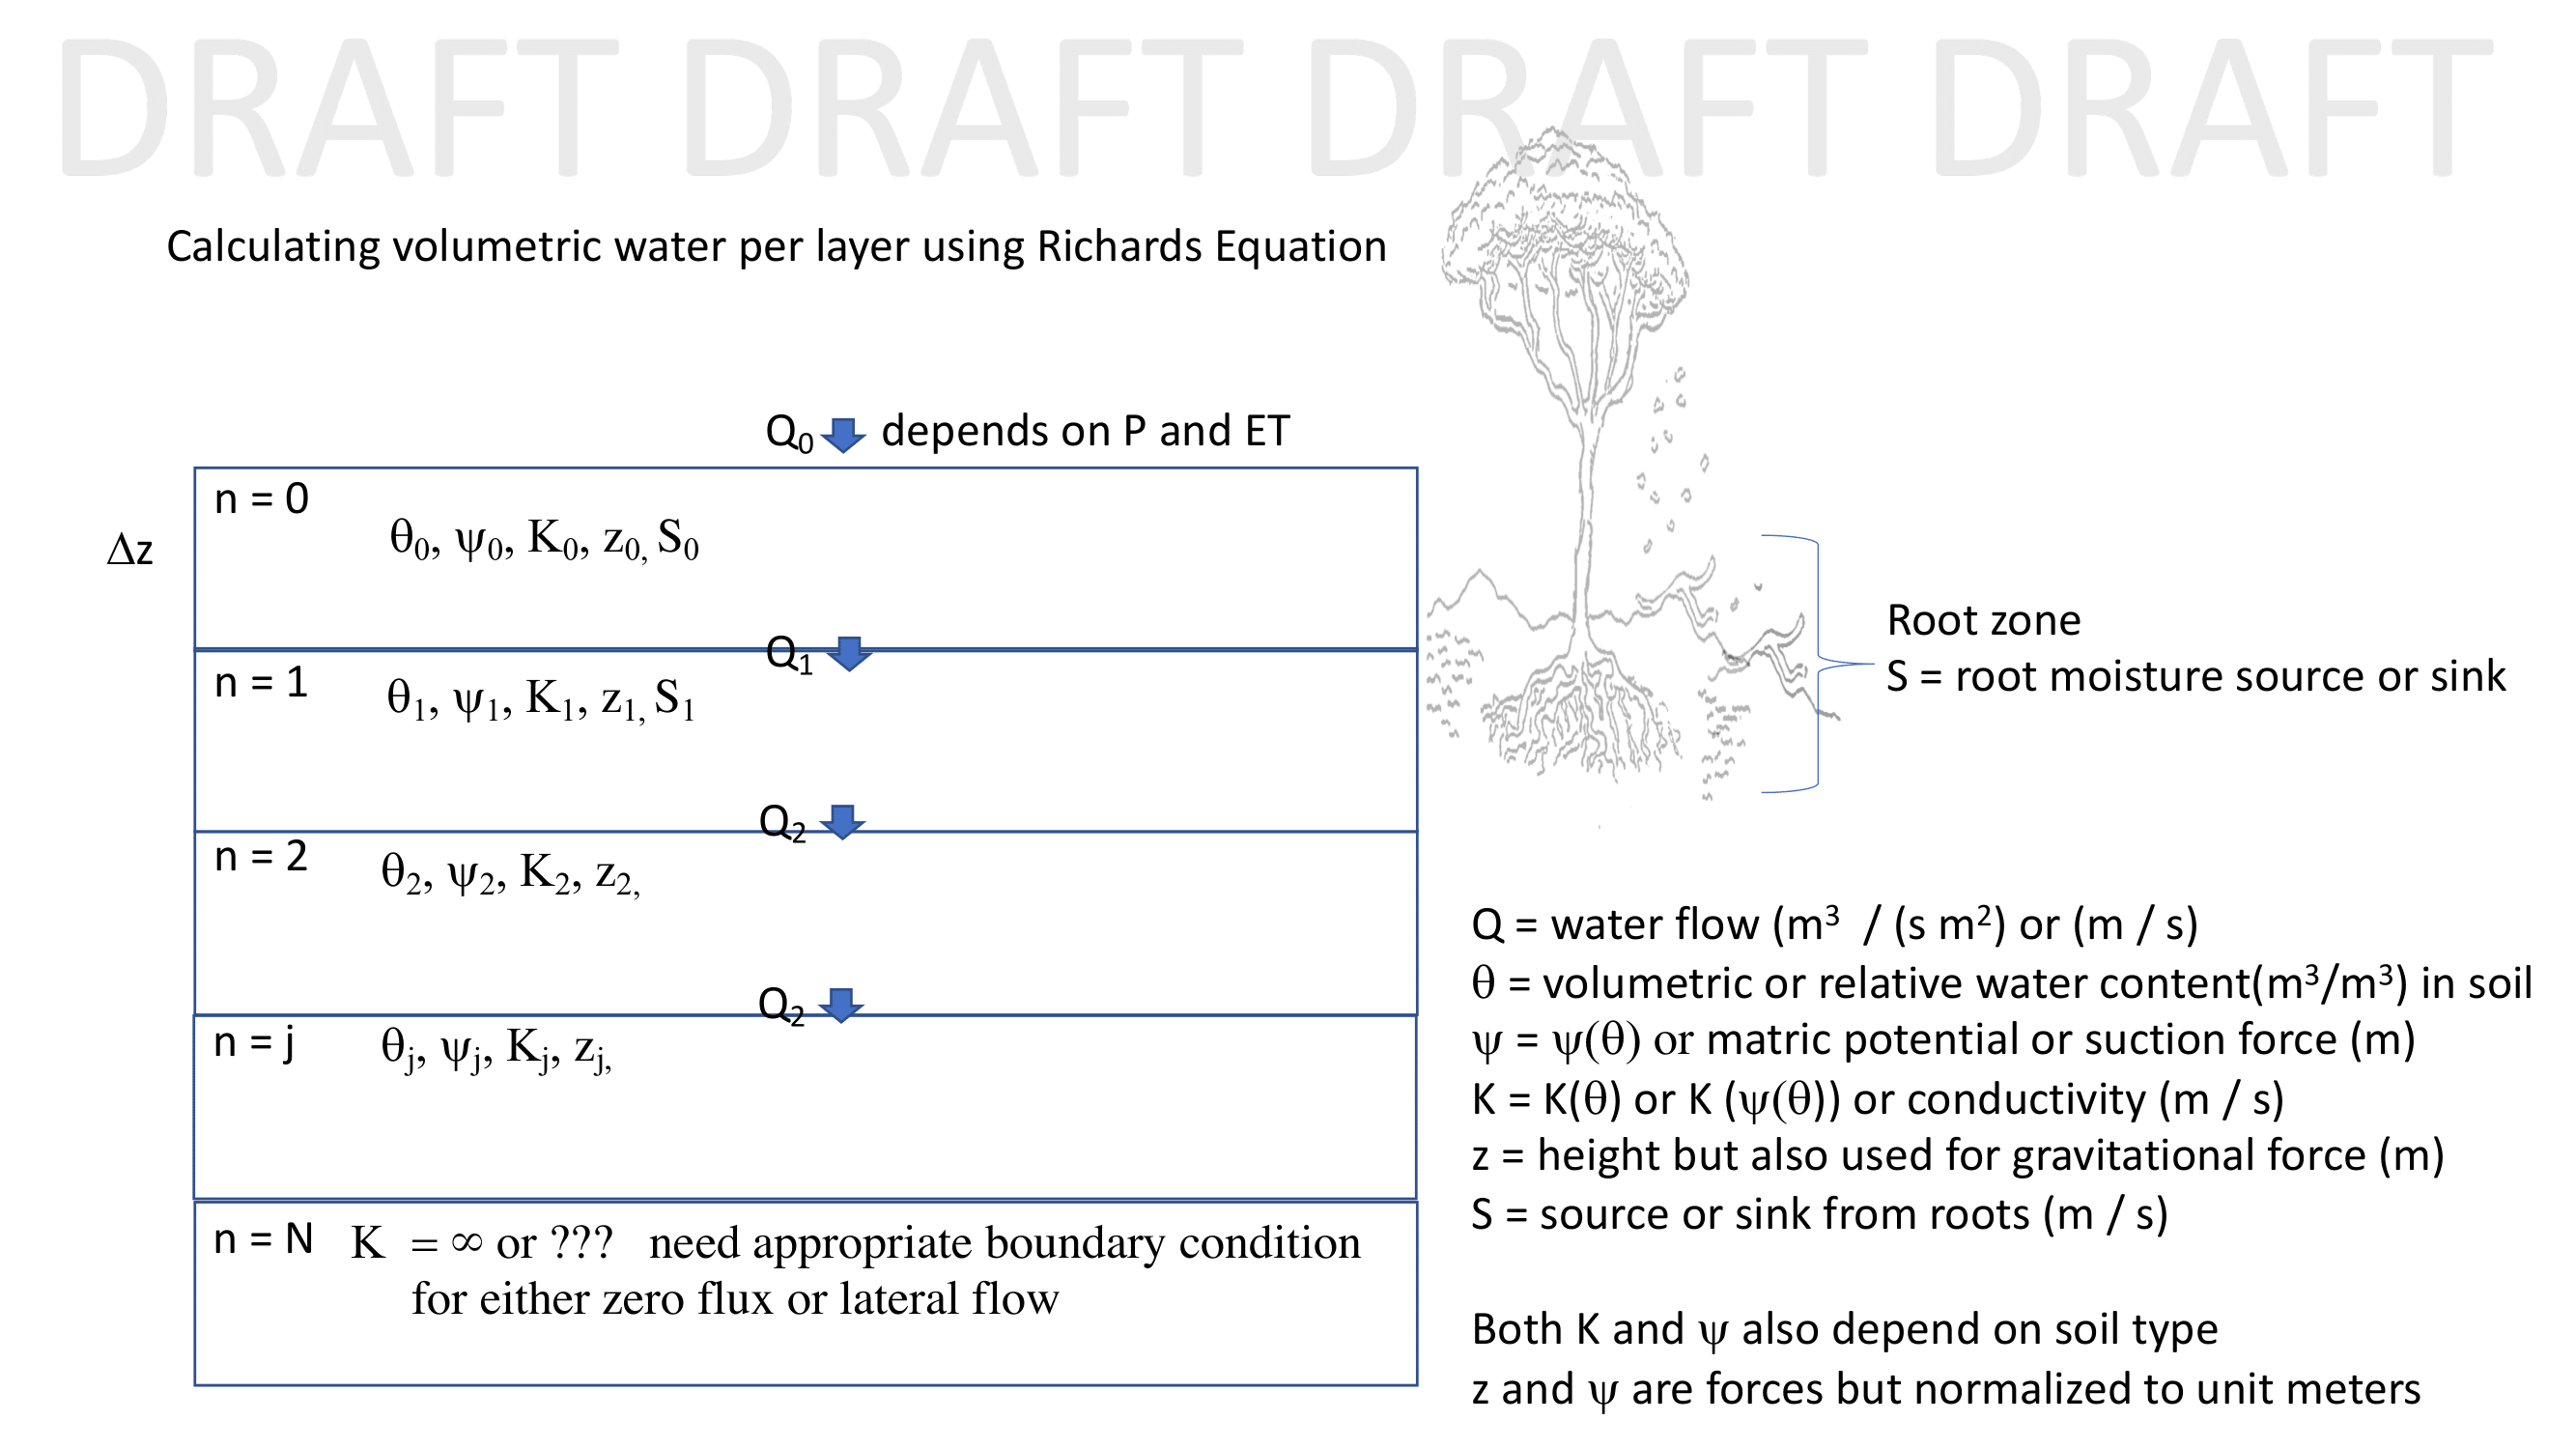
\includegraphics[scale=.15]{CLIMA-land/LM_figures/SoilSchematic-1.png}
\caption{Draft of soil schematic figure}
\end{figure}


\subsection{Phase Change}

The freezing of soil water or melting of soil ice releases or absorbs energy, respectively. Formation of ice releases latent heat, and temperature remains constant at the freezing point while soil water freezes. Similarly, melting of ice consumes energy, during which temperature does not increase. Latent heat of fusion is the amount of energy required to convert a unit of mass of frozen water to liquid. This transition requires 334 J g$^{-1}$. Freezing liquid water to ice releases a similar amount of energy. The total energy involved in phase change depends on soil moisture. For a volumetric water content $\theta$, the energy (J m$^{-3}$) required to freeze soil is $L_f \rho_{wat} \theta$, where $L_f =$ 0.334 MJ kg$^{-1}$ is the latent heat of fusion of water and $\rho_{wat} =$ 1000 kg m$^{-3}$ is the density of water. In course-grained soil such as sands, all the water present in the soil changes phase at a temperature close to 0$^{\circ}$C ($T_f =$ 273.15 K).  These soils can be treated with good approximation as either completely frozen or unfrozen. In fine-grain soils such as silts and clays, some soil water remains unfrozen even at temperatures below freezing. The amount of unfrozen water decreases as temperature decreases, and the latent heat release occurs over some temperature range $T_f - \Delta T_f$.

A simple way to account for freezing and thawing is to add the latent heat associated with phase change to the heat conduction equation to yield an apparent heat capacity \citep{lunardini1981heat}. Including a latent heat term as the unfrozen water $\theta_{liq}$ freezes, the heat conduction equation becomes
\begin{equation}
     c_v \frac{\partial T}{\partial t} = \frac{\partial }{\partial z} \left( \kappa \frac{\partial T}{\partial z} \right) - L_f \rho_{wat} \frac{\partial \theta_{liq}}{\partial t}.
\end{equation}
The second term on the right-hand side of the equation is a source of energy during freezing ($\partial \theta_{liq} / \partial t <$ 0) and is a sink of energy during melting ($\partial \theta_{liq} / \partial t >$ 0). The change in liquid water can be expressed as $\partial \theta_{liq} / \partial t = ( \partial \theta_{liq} / \partial T) (\partial T / \partial t)$, and the equation above can be re-written as 
\begin{equation}
     \left( c_v\ +\ L_f \rho_{wat} \frac{\partial \theta_{liq}}{\partial T} \right)  \frac{\partial T}{\partial t} = \frac{\partial }{\partial z} \left( \kappa \frac{\partial T}{\partial z} \right).
\end{equation}
Written this way, the term in parentheses on the left-hand side of the equation represents an effective heat capacity. Solution of this equation requires an expression for $\partial \theta_{liq}/{\partial T}$ to relate the amount of liquid water to temperature. In practice, however, the entire latent heat of fusion can be associated with a small finite temperature range between the freezing point and $T_f -\Delta T_f$ so that the effective heat capacity for a soil with water content $\theta$ is
\begin{equation}
c_v = \left\{
        \begin{array}{lll}
            c_{vu} & \quad T\ >\ T_f, \\
            c_{vf}\ + \frac{L_f \rho_{wat} \theta }{\Delta T_f} & \quad T_f - \Delta T_f\  \leq  T\ \leq\ T_f\ ,\\
            c_{vf} & \quad  T\ \leq\ T_f - \Delta T_f\\
        \end{array}
    \right.
\end{equation}
where $c_{vu}$ and $c_{vf}$ are the unfrozen and frozen volumetric heat capacity, respectively. The apparent heat capacity is the heat capacity of soil constituents plus a term that accounts for the latent heat of fusion. 

\begin{comment}

\hl{[The following is covered in Eq. (2.6) above.]} The heat capacity of air is negligible so that the heat capacity of soil is given by the weighted fraction of the heat capacity of solids, water and ice \citep{de1963thermal}, and
\begin{equation}
c_v = (1- \theta_{sat}) c_{v,sol} +  \theta_{liq} c_{v,wat} +  \theta_{ice} c_{v,ice}.
\end{equation}
The heat capacity of water is $c_{v,wat}= \rho_{wat}c_{wat} =$ 4.19 MJ m$^{-3}$ K$^{-1}$, for ice $c_{v,ice}= \rho_{ice}c_{ice} =$ 1.94 MJ m$^{-3}$ K$^{-1}$, and for soil solids $c_{v,sol} =$ 1.926 MJ m$^{-3}$ K$^{-1}$ \citep{de1963thermal}. The equation above can be applied assuming all water is either liquid or ice to calculate the unfrozen and frozen heat capacity, respectively.  

\end{comment}

Using the chain rule of differentiation and the fact that the matric potential is a monotonic function of $\theta_l$, Darcy's law can also be written as
\begin{equation}\label{e:darcy_law2}
    \vec{\tilde d}_l = - K(\theta_l) \left(C_l(\theta_l)^{-1} \grad\theta_l + \grad \psi_z \right),
\end{equation}
where
\begin{equation}
C_l(\theta_l) = \left( \frac{d\psi}{d\theta_l} \right)^{-1} =   \frac{d\theta_l}{d\psi} 
\end{equation}
is known as the specific moisture capacity ($\mathrm{m^{-1}}$). The last equality is the derivative of the inverse $\theta_l(\psi)$ of the function $\psi(\theta_l)$, which is commonly used in hydrology and is known as the water retention curve. The quantity $K(\vec{\theta})/C(\vec{\theta})$ has units of diffusivity ($\mathrm{m^2~s^{-1}}$) is known as the soil water diffusivity. It is singular where the specific moisture capacity $C(\theta_l)$ is zero, which is the case in saturated soil. 

Integrating the water balance equation \eqref{e:soil_water_conservation} numerically is challenging primarily because of this singularity at the water table, where the unsaturated (vadose) zone meets the saturated zone \citep{Farthing17a}.

\subsection{Summary of soil heat and moisture equations for CliMA implementation}

This section contains a summary of all equations needed for implementation of the soil heat and moisture equations into CliMA. All variables are defined 

[OPTION: list equations in table for succinct description and avoid extra equation numbers in document] \\

\textbf{Soil Heat Equation} \\


\begin{equation}
     \frac{\partial (\rho_s c_s T_s) }{\partial t} = \frac{\partial }{\partial z}\kappa \frac{\partial T_s }{\partial z}
\end{equation}

\begin{equation}
    f_{\mathrm{om}} = \rho_{\mathrm{om}}/\rho_{om,{\rm max}}
\end{equation}


\begin{equation}
\kappa = K_e \kappa_{\rm sat} + (1-K_e) \kappa_{\mathrm{dry}}
\end{equation}

\begin{equation}
K_e = \exp \big( \gamma((1-s(\gamma-1.33))\big)
\end{equation}

\begin{equation}
s=\theta/\theta_{\rm sat}
\end{equation}

\begin{equation}
c_s=\theta c_{\rm liq} + (1-\theta) c_{\rm dry}
\end{equation}

\begin{equation}
c_{\rm dry} = (1-f_{\mathrm{om}})c_{soil} + f_{\mathrm{om}}c_{\mathrm{om}}
\end{equation}

\begin{equation}
c_{soil} = {\rm \frac{2.128 (sand)+ 2.385 (clay)}{(sand) + (clay)}}
\end{equation}  \\



\textbf{Soil Moisture Equations} \\

(Unsaturated soil)
\begin{equation}
 dS=d\theta 
\end{equation}

(Saturated - Unconfined Aquifer)
\begin{equation}
 dS=S_y dh ; S_y = n
\end{equation}

(Saturated - Confined Aquifer)
\begin{equation}
 dS=S_s dh
\end{equation}

\begin{equation}
 h=z+\psi
\end{equation}

\begin{equation}
dS = C(\psi)d\psi
\end{equation}

(Unsaturated soil)
\begin{equation}
C(\psi)=\partial \theta /\partial h 
\end{equation}

(Unconfined aquifer)
\begin{equation}
C(\psi)=S_y 
\end{equation}

(Richards' equation)
\begin{equation}
     \frac{\partial S}{\partial t} = C(\psi)\frac{\partial \psi}{\partial t} = -\nabla \cdot {\bf{q}} + {\rm Source}
\label{Richards}
\end{equation}

\begin{equation}
     \bf{q} = - \mathbf{K}(\psi) \otimes \nabla h
\end{equation}

(Unsaturated zone)
\begin{equation}
     \frac{\partial \theta}{\partial \psi}\frac{\partial h}{\partial t} = \frac{\partial}{\partial z} \left( {K(\psi)\frac{\partial \psi}{\partial z}} + 1 \right) + {\rm Source}
\end{equation} \\

(Saturated - Unconfined Aquifer)
\begin{equation}
     \frac{\partial S}{\partial t} = S_y \frac{\partial h}{\partial t} = \nabla \cdot \left( {K_{\rm sat} \nabla h} \right) + {\rm Source}
\end{equation} \\


\textbf{Retention functions for unsaturated soils - van Genuchten} \\


\begin{equation}
     \theta(\psi) = \theta_{\mathrm{res}} + \frac{\theta_{\mathrm{sat}} - \theta_{\mathrm{res}}}{\left[ 1+(\alpha |\psi|)^n \right]^{m}}
\end{equation}

\begin{equation}
m=1-1/n
\end{equation}

\begin{equation}
     K(\psi) = K_{\mathrm{sat}} S_e^L \left (1 -  (1-S_e^{1/m})^m  \right)^2
\end{equation}

\begin{equation}
L = 0.5
\end{equation}

\begin{equation}
     S_e = \frac{\theta(\psi) - \theta_{\mathrm{res}}}{\theta_{\mathrm{sat}} - \theta_{\mathrm{res}}}
\end{equation}

\begin{equation}
     \frac{\partial \theta}{\partial \psi} =   \frac{m n\alpha^n |\psi|^{n-1}}{\left[ 1+(\alpha |\psi|)^n \right]^{m+1}} \left( \theta_{\mathrm{sat}} - \theta_{\mathrm{res}} \right) 
\end{equation}


\subsubsection{Retention curves $\theta=f(\psi)$ and $K(\psi)$ in the unsaturated zone}
\label{SoilMoisture:Retention_Curves}
    {\bf Van Genuchten} \\
We will use the van Genuchten formulation as a reference retenstion curve, as it is better behaved in saturated conditions than the Brooks and Corey relationship 
\begin{equation}
     \theta(\psi) = \theta_{\mathrm{res}} + \frac{\theta_{\mathrm{sat}} - \theta_{\mathrm{res}}}{\left[ 1+(\alpha |\psi|)^n \right]^{m}}
\end{equation}
with $m=1-1/n$.
For hydraulic conductivity, we have
\begin{equation}
     K(\psi) = K_{\mathrm{sat}} S_e^L \left (1 -  (1-S_e^{1/m})^m  \right)^2
\end{equation}
with $L$ an empirical parameter assumed to be $L=0.5$. $S_e$ is the relative degree of saturation of the soil and $K_{\mathrm{sat}}$ the hydraulic conductivity at saturation. 
\begin{equation}
     S_e = \frac{\theta(\psi) - \theta_{\mathrm{res}}}{\theta_{\mathrm{sat}} - \theta_{\mathrm{res}}}
\end{equation}
The derivative of $\theta$ with respect to $\psi$, $C(\psi)$ is:
\begin{equation}
     \frac{\partial \theta}{\partial \psi} =   \frac{m n\alpha^n |\psi|^{n-1}}{\left[ 1+(\alpha |\psi|)^n \right]^{m+1}} \left( \theta_{\mathrm{sat}} - \theta_{\mathrm{res}} \right). 
\end{equation}


    {\bf Brooks and Corey} \\
An alternative approach to Van Genuchten will be to use the Brooks-Corey relationships:
\begin{equation}
     \theta(\psi) = \theta_{\mathrm{res}} + (\theta_{\mathrm{sat}} - \theta_{\mathrm{res}})\left( \frac{\psi}{\psi_{ae}}\right)^{-\lambda}
\end{equation}
with $\psi_{ae}$ the air entry point.
\begin{equation}
     K(\psi) = K_{\mathrm{sat}} \left( \frac{\psi}{\psi_{ae}}\right)^{-2-3\lambda}
\end{equation}


% Calculation of Kersten number and kappa_s for Thermal Conductivity calculation 
\begin{comment}
For unfrozen soil: \hl{[what is this based on? does it have a strong basis in global data?]}
\begin{equation}
K_e = \left\{
        \begin{array}{ll}
            1.0 + 0.7\ \mathrm{log_{10}}\ S_e & \mathrm{course-texture\ soil\ } (S_e > 0.05), \\
            1.0 + \mathrm{log_{10}}\ S_e & \mathrm{fine-texture\ soil\ } (S_e > 0.10)
        \end{array}
    \right.
\end{equation}
and fine-texture soil has a sand content of less than 50\%. For frozen soil:
\begin{equation}
K_e = S_e.
\end{equation}
In these equations, $S_e= \frac{\theta}{\nu_p}$ is the relative wetness, with $\theta$ as the volumetric water content (m$^{3}$ H20 m$^{-3}$ soil) and $\nu_p=\theta_{sat}$ as the volumetric water content at saturation (also equal to porosity). 

The dry and saturated thermal conductivities depend on soil properties. The thermal conductivity of dry soils varies with bulk density (kg m$^{-3}$) according to 
\begin{equation}
\kappa_{\mathrm{dry}} = \frac{ (0.135 \rho_\mathrm{b} + 64.7 )}{ (2700 - 0.947 \rho_\mathrm{b} )}.
\end{equation}
where $\rho_\mathrm{b} = 2700(1- \theta_{sat})$ and 2700 kg m$^{-3}$ here represents the density of soil solids. The thermal conductivity of saturated soil is calculated from the thermal conductivity of the components (solids $\kappa_{solids}$, water $\kappa_{liquid}$, and ice $\kappa_{ice}$) and their respective volume fractions. For unfrozen soil:
\begin{equation}\label{e:conductivity_sat}
\kappa_{\mathrm{sat}} = \kappa_{solids}^{(1- \theta_{sat} )}  \kappa_{liquid}^{(\theta_{sat} )}. 
\end{equation}
And for frozen soil:
\begin{equation}
\kappa_{\mathrm{sat}} = \kappa_{solids}^{(1- \theta_{sat} )}  \kappa_{ice}^{(\theta_{sat} )}. 
\end{equation}
A general expression allowing a mixture of liquid water and ice is
\begin{equation}
\kappa_{\mathrm{sat}} = \kappa_{solids}^{(1- \theta_{sat} )}  \kappa_{liquid}^{(f_u \theta_{sat} )}  \kappa_{ice}^{( (1-f_u) \theta_{sat} )}.
\end{equation}
This equation recognizes that even at temperatures below freezing, the total water consists of unfrozen $\theta_{liq}$ and frozen $\theta_{ice}$ water ($\theta = \theta_{liq} + \theta_{liq}$), and $f_u = \frac{\theta_{liq}}{\theta}$ is the fraction of the total water that is unfrozen. Representative values are $\kappa_{liquid} = 0.57$ W m$^{-1}$ K$^{-1}$ and $\kappa_{ice} = 2.29$ W m$^{-1}$ K$^{-1}$. 
The thermal conductivity of a soil varies with the quartz content of the soil. The Johansen method described by \citep{Farouki81a} gives an approximation of such a dependence on quartz content:
\begin{equation}
\kappa_{solids} = \kappa_{q}^q \kappa_{o}^{1-q},
\end{equation}
where $q$ is the quartz content as a fraction of the total soil solids, $\kappa_{q}$ = 7.7 W m$^{-1}$ K$^{-1}$ is the thermal conductivity of quartz, and $\kappa_{o}$ = 2.0 W m$^{-1}$ K$^{-1}$ is the thermal conductivity of other minerals for soils with $q >$ 0.2 and  $\kappa_{o}$ = 3.0 W m$^{-1}$ K$^{-1}$ for $q <=$ 0.2. The accuracy of this equation depends on the specified thermal conductivity of quartz and the quartz fraction. The quartz content can be approximated by the sand content (i.e. quartz fraction $q$ $\sim$= fraction of soil that is sand)  \citep{peters1998effect}, though this is not necessarily correct \citep{lu2007improved}.  
\end{comment}


% Old Explanation of Calculation of Kersten number and kappa_s for Thermal Conductivity calculation
\begin{comment}
The thermal conductivity of soil depends on the water content and is modeled as a weighted mean of a conductivity $\kappa_{\mathrm{dry}}$ of dry soil and a conductivity $\kappa_{\rm sat}$ of water-saturated soil,
\begin{equation}\label{e:soil_conductivity}
\kappa = K_e \kappa_{\mathrm{sat}} + (1-K_e) \kappa_{\mathrm{dry}}.
\end{equation}
The weighting factor $K_e$ is the Kersten number, which is function of soil relative humidity $s=\theta/\theta_{\rm sat}$. (However, the thermal diffusivity $\kappa/\tilde c_s$ has a much weaker moisture dependence than $\kappa$ itself because of a compensation of the moisture dependence between $\kappa$ and $\tilde c_s$.)

The saturation heat conductivity, even in the presence of frozen ground, can be expressed as a function of the ice and liquid water contents assuming a geometric mean: \hl{[why do we average geometrically here and arithmetically above? Seems odd.]}
\begin{equation}\label{e:conductivity_sat}
\kappa_{\mathrm{sat}} = \kappa_{solids}^{(1- \theta_{sat} )}  \kappa_{liquid}^{(f_u \theta_{sat} )}  \kappa_{ice}^{( (1-f_u) \theta_{sat} )} 
\end{equation}
where $\kappa_{\mathrm{sat}}$ is the thermal conductivity of a saturated soil, and is calculated from the thermal conductivity of the components ($\kappa_{solids}$, $\kappa_{liquid}$, and $\kappa_{ice}$), $\theta_{sat}$ is the volumetric water content at saturation (also equal to porosity), and $f_u = \theta_{liquid} / \theta$ is the fraction of total water that is unfrozen. Representative values are $\kappa_{liquid} = 0.57$ W m$^{-1}$ K$^{-1}$ and $\kappa_{ice} = 2.29$ W m$^{-1}$ K$^{-1}$. 
The thermal conductivity of a soil varies with the quartz content of the soil. The Johansen method described by \cite{Farouki81a} gives an approximation of such a dependence on quartz content:
\begin{equation}
\kappa_{solids} = \kappa_{q}^q \kappa_{o}^{1-q}
\end{equation},
where $q$ is the quartz content as a fraction of the total soil solids, $\kappa_{q}$ = 7.7 W m$^{-1}$ K$^{-1}$ is the thermal conductivity of quartz, and $\kappa_{o}$ = 2.0 W m$^{-1}$ K$^{-1}$ is the thermal conductivity of other minerals for soils with $q >$ 0.2 and  $\kappa_{o}$ = 3.0 W m$^{-1}$ K$^{-1}$ for $q <=$ 0.2.
\end{comment}
